% TODO: footnotes (now missing)
% TODO: in-text formatting (e.g., \textit, quotes)
% TODO: bibliography
% TODO: font-size listings in appendices. blue formatting for values
% TODO: appendices not numbered like this... (how else?)


\chapter{Evoke: Exploring and Extending \emph{A Thesaurus of Old English} using a Linked Data Approach}
\chaptermark{Evoke}

\begin{abstract}
This article provides an introduction to the web application Evoke. This application offers functionality to navigate, view, extend, and analyse thesaurus content. The thesauri that can be navigated in Evoke are expressed in Linguistic Linked Data, an interoperable data form that enables the extension of thesaurus content with custom labels and allows for the linking of thesaurus content to other digital resources. As such, Evoke is a powerful research tool that facilitates its users to perform novel cultural linguistic analyses over multiple sources. This article further demonstrates the potential of Evoke by discussing how \textit{A Thesaurus of Old English} was made available in the application and how this has already been adopted in the field of Old English studies. Lastly, the author situates Evoke within a number of recent developments in the field of Digital Humanities and its applications for onomasiological research.
%\keywords{Evoke, onomasiology, Old English, Digital Humanities, A Thesaurus of Old English, Linguistic Linked Data}
\end{abstract}


\section{Introduction}
\label{sect:intro}

Vocabulary has been described as “a very sensitive index of the culture of a people” (Sapir, 1963: 27). This notion forms the corner stone of cultural linguistics, which explores the relationship between language and culture (Sharifian, 2015: 515). Examining which words are (or were) available to a language community can offer valuable insights into their culture (Hough and Kay, 2017). Moreover, the word choices made \textit{within} such a community can shed light on a number of aspects, including the intentions of speakers and authors, as well as their conscious or unconscious preferences.\footnote{See also the contributions by Amos van Baalen and Thijs Porck in this special issue.}  Lexicographical works known as thesauri capture information about the lexicon and are veritable treasure troves for exploring the vocabulary of a language community and its relation to their culture.

A thesaurus is a lexicographic resource that organizes words and phrases according to their meaning rather than alphabetically.\footnote{For further detail on this type of lexicographical work, and the distinction with other common senses of the word \textit{thesaurus}, we refer the reader to Hartmann (2006) and Kay and Alexander (2016).}  Its overarching structure consists of a hierarchy of semantic concepts (Kay and Roberts, 1994). Concepts that represent abstract or generic meanings in this tree-like structure branch out to ones that are increasingly specific in meaning.\footnote{This structure, used to categorize lexical material, is not unlike the taxonomies of animals and plants created by Carl Linnaeus (1707-1778).}  Each of these concepts can act as a category for words and phrases that express its meaning.\footnote{To be precise, thesauri categorize words and phrases in a given \textit{sense} (Hüllen, 1999: 13).}  Thus, the semantic hierarchy of a thesaurus allows users to move from meaning to lexical item. This process can be illustrated with \textit{A Thesaurus of Old English}, which allows users to look up early medieval English words by means of its semantic hierarchy (which it indicates through strings of numbers). An example of one of the most generic meanings in its hierarchy is the concept “12 Power, might”. From this concept, it is possible to navigate branches down the hierarchy. One of these branches leads, via the more specific concepts “12.01 Power, control, sway” and “12.01.01 Authority”, to the concept “12.01.01.10 Freedom, being free”. Here, the thesaurus indicates which Old English words express this meaning: \textit{frēols} and \textit{frēot}.

It is self-evident that one of the main uses of thesauri is to look up alternative phrasings (e.g., Old English frēols or frēot to express ‘freedom, being free’).  However, owing to its semantic hierarchy, a thesaurus offers several other opportunities for research (Brewer, 2010: 802; Adamska-Sałaciak, 2010: 232; Busse, 2012: 88).  These opportunities include exploring whether a word exists for a certain semantic concept; the number of words that express that concept (known as the degree of lexicalization or cultural elaboration) (Wierzbicka, 1997: 10-11); the number of words and nuances available within a given semantic domain; which semantic domains are related through the various senses of a word (i.e., through polysemy); and how generic or specific the meaning of a word or group of words is. Traditionally, the acquisition of this kind of information from a thesaurus has relied on manual labour: leafing through paper editions of thesauri to find sections of relevance,  or manually counting the number of words presented on a website.  The web application Evoke (Stolk, 2018) introduces a user-friendly interface that allows researchers to digitally explore thesaurus content, enrich existing thesauri with additional knowledge, and analyse combined content in order to obtain semantic fingerprints that we call ‘onomasiological profiles’.

The current version of Evoke (version 1.4.1) offers functionality to navigate, view, extend, and analyse thesaurus content.  The software facilitates users in answering such cultural linguistic questions as ‘which words were available to a certain culture?’, ‘what is the degree of lexicalization of a concept’ and ‘which other notions were associated with a given word (owing to polysemy and homonymy)?’ Moreover, thesauri that can be navigated in Evoke are expressed in an interoperable data form: Linguistic Linked Data (Cimiano et al., 2020). This form adheres to a number of best practices for data (Wilkinson et al., 2016; Lóscio et al., 2017) and employs standardized and interoperable data vocabularies for the Semantic Web (Miles and Bechhofer, 2009; Cimiano, McCrae and Buitelaar, 2016). In effect, this data form enables the extension of thesaurus content in Evoke with custom labels, facilitates linking thesaurus content to other digital resources, and allows novel analyses to be performed over multiple sources. 

This article describes the development of Evoke and how it has been used to further explore A Thesaurus of Old English, which is the first thesaurus to be made available for analysis within this application. Sections 2 to 4 outline the requirements this web application had to meet in order to facilitate research into thesauri, its operating architecture, and the functionality it currently offers. Next, sections 5 and 6 discuss how A Thesaurus of Old English has been made available in a Linguistic Linked Data form and how researchers have been able to use Evoke to further explore this resource. Lastly, section 7 contrasts Evoke with existing software and discusses how Evoke and related work in the field of Digital Humanities may impact the future of onomasiological and cultural linguistic research. 


\section{Requirements}

In order to facilitate research into thesauri, the first step in making Evoke was to gauge the research needs that it could answer. On the basis of published reviews of thesauri as well as a number of research cases, five requirements were established that the new web application had to meet. The first three requirements (R1-R3) were gathered for the first version of Evoke. The remaining two requirements (R4-R5) were formulated for subsequent iterations of the application and were collected from stakeholders – experts in lexicography, linguistics and philology (amongst other fields) – to ensure that the software is intuitive and useful for both research and educational purposes. Stakeholder requirements were gathered by several means: dedicated stakeholder meetings, workshops, and feedback based on preliminary results in research and education projects. Additionally, requirements on the architecture (AR1-AR3) were based on best practices for data on the Web, transparent data management, and limitations imposed by licensing schemes of existing lexicographic resources.

\textbf{R1. Navigation.} A thesaurus can be approached in two manners: through its overarching taxonomy or through the lexis it organises (HTOED: ix). Both means are deemed key in allowing users – both newcomers and frequent users – to navigate the lexicographic content (Kay and Alexander, 2016: 368). 

\textbf{R2. Resource views.} Complete overviews of available information are to be presented on any given resource within a thesaurus that a user chooses to inspect. These overviews must indicate relations to other resources where relevant, such as listing the words that are allocated to the viewed location of the thesaurus taxonomy, or indicating the various branches of the taxonomy that contain one of the senses of the currently inspected word or phrase.

\textbf{R3. Extension.} The application should allow users to extend a thesaurus, connecting additional information to its content (cf. Bremmer, 2002: 111; Görlach, 1998: 399; Dance, 1997: 313; Kay, 1996: 72). Examples of such extensions are indications of date and dialect, results from corpus searches, and indications whether a word or meaning is found in a particular text, context, or is notable in some other qualitative or quantitative way. This functionality offers users the means to have the thesaurus reflect their own interests and to share salient information with others.

\textbf{R4. Analyses.} Thesauri are valuable for investigations into a range of aspects encoded in the lexicon: cultural elaboration, semantic domains and their cultural connotations, stylistic preferences of authors, use and development of metaphors, and so on (e.g., Spevack, 1993; Crystal, 2014; Anderson, Bramwell, and Hough, 2016; Porck, 2016: 59-71, 239-294; Diller, 2017). Statistical analyses, utilizing the onomasiological structure of the thesaurus and features of the lexis it contains, are therefore a key functionality.

\textbf{R5. Data management.} Proper data management should be an essential aspect of the application in facilitating onomasiological research. Users must have full control over their own data (e.g., creating backups, sharing their data with others) and the ability to select which data sources are deemed relevant for their explorations, allowing sets of information to be combined for viewing and analysis.

\textbf{AR1. Interoperable data form.} The software is to read and display resources published as Linguistic Linked Data. This vocabulary, and the underlying data format (RDF), facilitate reuse and interoperability of linguistic resources according to the FAIR data principles (Wilkinson et al., 2016; Lóscio et al., 2017). 

\textbf{AR2. Decentralized data.} The software must be capable of accessing data stored in a decentralized manner rather than relying on a central database, thereby stimulating a separation of data storage and services. Such separation is intended to remove barriers in selecting alternative solutions on both fronts, i.e., where the data is hosted and which application suits the needs of the user best (Verborgh, Wrigley, and Ballardini, 2019).

\textbf{AR3. Support limited licenses.} It is not uncommon to find lexicographic resources subject to licenses meant for viewing only, stipulating that users are not allowed to copy or download a substantial portion of the entire resource.  A Thesaurus of Old English is one such work. The architecture of the application must allow interacting with and extending resources that are available under a license limiting access to browsing, in addition to those available under fully open access.

The eight requirements listed above (R1-R5 and AR1-AR3) have informed the design of Evoke, which will be discussed in the next two sections. These sections, on the architecture and functionality of the application, will reference requirements that are relevant for the design element under discussion.

\section{Architecture of Evoke}

Evoke has been designed as a web application, which, when accessed, runs in the user’s internet browser. The application loads linguistic data from available data services and employs client-side rendering to display that information; rather than fetching an entire new webpage from a server whenever the user navigates to a different section, the application fetches only data necessary (linguistic data, in this case) to fill out pages that it itself composes locally (Scott, 2015). Code for navigating Evoke is therefore executed on a user’s computer rather than on a server dedicated to this purpose, resulting in a thin server architecture. As a result, Evoke demands server capabilities for hosting static files only (i.e., the web application) instead of additionally offering more advanced rendering technologies. The smaller demand on server-side resources should, in the case of Evoke, reduce hosting costs for the application. The code libraries used to render the interface of Evoke client-side are React and Reactstrap (basic HTML) complemented by ones specifically intended for vector graphics (i.e., D3, D3Pie, Recharts, and Wordcloud).  

\subsection{Linguistic Linked Data}
The data form supported by Evoke for accessing, exploring, and extending content is Linguistic Linked Data (cf. AR1) (Cimiano et al., 2020). This data form adheres to a number of best practices for data (Wilkinson et al., 2016; Lóscio et al., 2017) and employs standardized and interoperable data vocabularies for the Semantic Web (Miles and Bechhofer, 2009; Cimiano, McCrae, and Buitelaar, 2016). The Linguistic Linked Data paradigm builds on Linked Data principles, which advocate the use of Web mechanisms for capturing and sharing data, employing graph-based models (i.e., nodes and relations between them) and identifying data by means of IRIs (often Web addresses) (Cimiano et al., 2020). The use of IRIs allows one to capture and identify data in a language-independent manner, reuse terminology defined elsewhere, and to create links between datasets or nodes within different datasets. In effect, this data form enables thesaurus content in Evoke to be extended with custom labels and links to other digital resources.

Applying Linked Data principles to language resources nets a number of benefits (Chiarcos et al., 2013). One of these benefits is that their data form enables the merging of datasets in order to obtain a valid combined set of data. Thus, linguistic resources and datasets elaborating on them can be queried in unison. A second benefit is an increased level of interoperability. Using standardized terminology in describing linguistic data increases a shared understanding of that data and facilitates their interpretation by software. Moreover, the use of IRIs as identifiers ensures data can be linked without the need for duplication of information from one dataset into the other. The ability to link (or reference) in such a manner is valuable in the setting of Linguistic Linked Data, since it is not uncommon to find lexicographic resources subject to licenses meant for viewing only, stipulating that users are not allowed to copy or download a substantial portion of their content (e.g., OED Online and HTE). By adopting IRIs in published lexicographic resources, their users can explore and extend these resources, engaging with the content offered, without infringing on such licenses (cf. AR3).

The Evoke web application, in order to draw on the aforementioned benefits, assumes language resources to adopt Linguistic Linked Data as specified by the W3C OntoLex community (Cimiano, McCrae, and Buitelaar, 2016), applied specifically to the context of topical thesauri (Stolk, 2019). Other resources can be viewed and extended in Evoke, too, as long as they are formulated using the same syntax that underlies Linguistic Linked Data: RDF (Cyganiak, Wood, and Lanthaler, 2014). Thus, Evoke can work with non-linguistic data connected to thesauri as well as future modules put forward by the OntoLex community for Linguistic Linked Data (such as that supporting frequency and attestations) (Chiarcos et al., 2020). The use of RDF in Evoke is not limited to solely the content of datasets available, as will be discussed in sections 3.3 and 3.4.

\subsection{Accessing Datasets}
The architecture of Evoke offers a high degree of flexibility in managing which content is to be viewed or analysed, including where individual datasets have been made available. The functionality to realize this hinges on the use of so-called data catalogues, which list available datasets and the data services supplying them. Upon start-up, Evoke loads a default data catalogue that, at the time of writing this article, contains the Linguistic Linked Data version of A Thesaurus of Old English (see section 5) and the datasets created through novel research presented in this special issue (e.g., Beowulf Thesaurus; Andreas Thesaurus; Old English Martyrology Thesaurus; Ælfrician Vocabulary; and Old Frisian Kinship). Custom data catalogues can, however, be used too.

\begin{figure}[htbp]
	\framebox[\textwidth]{
		\scalebox{0.45}[0.45]{
			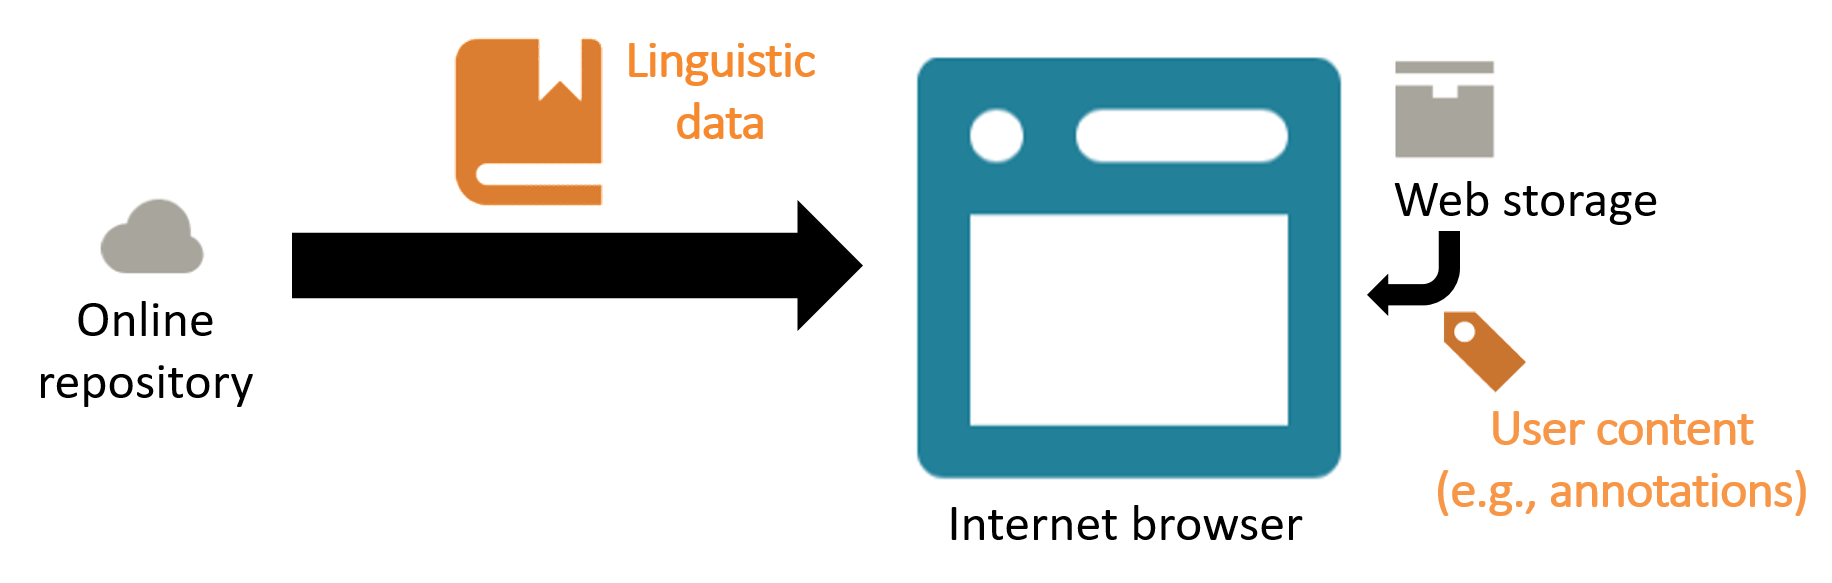
\includegraphics{Stolk2021a/fig/Fig1.png}
		}
	}
	\caption[]{\label{fig:Stolk2021a:Fig1} Sources of data that Evoke retrieves and presents.}
\end{figure}

Datasets listed in a catalogue are accessed through asynchronous calls to SPARQL endpoints and/or APIs (cf. the online repository in Fig. 1). As data is retrieved through such calls in the background, the Evoke web application contains a so-called high-order component that acts as loader. This loader wraps the component that is to be presented, but still void of data, in another component that first awaits data requests. During the loading time, a loading icon is presented. Once the data required has been retrieved, the loader renders the wrapped component with its proper input. This mechanism is used, in combination with the underlying data form of Linguistic Linked Data, to follow links iteratively in fetching further information from all datasets that are to be accessed. Thus, when a user selects a semantic concept of a thesaurus for viewing, a list of words that express that concept is retrieved. For each of those words, their IRI (i.e., their identifier) is subsequently used to collect all associated labels available across the datasets – whether they are part of the original thesaurus data or a set of annotations created by others.

The application reads, next to data served remotely via SPARQL or API calls, Linked Data stored in the user’s internet browser (cf. the Web storage in Fig. 1). A dataset in the browser can be stored using either the Turtle serialization or in JSON-LD and is interpreted using libraries from the Comunica framework (Taelman et al., 2018).  The use of this storage method in Evoke is detailed in section 4.3.

\subsection{Data Catalogue}
The data catalogues in Evoke adhere to the W3C DCAT vocabulary, an international standard developed specifically for expressing datasets and the services that provide these sets, including access details (Albertoni et al., 2020). This information is stored in the JSON-LD format and can therefore be read as JSON or, through the context provided, interpreted as RDF (Sporny et al., 2020). The use of these standards are meant to accommodate a higher level of interoperability with other tooling and services. An example catalogue is shown in Appendix 1. Drawing from a catalogue, the user interface of Evoke provides the means to select which available datasets are to be explored in unison (cf. R5, see Fig. 9). Users can add their own datasets or data services to a catalogue, store their catalogue locally as a JSON file, and activate a local catalogue by dragging and dropping it onto the Evoke web application. 
Access to datasets may or may not need to be limited, depending on the usage license associated with them. In order to ensure that Evoke can work with more restrictive licenses (cf. AR3), two types of access mechanisms for data services are supported in data catalogues: (1) a SPARQL endpoint and (2) the Evoke API. The former allows services to respond to any query using the standardized querying language for RDF. The latter ensures content can be viewed and browsed in Evoke through a basic set of queries specific for this need, without offering users full access (that is, the possibility to extract or download the full dataset).  Distinguishing between these two types of access mechanism in the data catalogue is achieved through different values for the endpointDescription attribute of data services. 
Which datasets listed in the active catalogue will be queried by Evoke depends on the selection made by the user. The Evoke interface allows users to enable (or disable) datasets listed. Only those datasets can be enabled that (1) have a data service associated with them and (2) already have all of their required dependencies enabled. To illustrate, the ‘Riddle 47’ dataset contains links to the dataset ‘A Thesaurus of Old English’ and depends on it for analyses. Once a user has enabled this required dataset in the interface, that user can opt to enable the ‘Riddle 47’ dataset, too (see the top bars in Fig. 9). Datasets served by the same service, though available in different graphs, are queried in unison and allow statistical analyses to be performed. 

\subsection{Browser Storage}
Any user of the Evoke web application can annotate linguistic content, such as words or semantic concepts, with information relevant to them. Typing a sentence in the annotation component of a page will automatically create a Linked Data annotation that adheres to the Web Annotation standard of W3C (Sanderson, Ciccarese, and Young, 2017), including any extracted label when a hashtag is used (see “\#riddle47” in Fig. 10). The novel aspect of this approach is that such an annotation is not stored in an online database, but is instead stored locally in the user’s internet browser, employing the localStorage attribute of Web storage (cf. AR2) (Hickson, 2016). Annotations stored in the browser can be downloaded as a file to backup (see Appendix 2) and can be reactivated in the browser — giving users full control over their created content and allowing them to share it in the manner of their choosing (cf. R5). Publishers of the original lexicographic resource benefit from this approach, too, as they neither need to moderate, store, or host annotations, nor offer users login mechanisms before they can interact with the information. Costs for hosts may thus be substantially reduced for presenting users with this functionality.

Annotations contain references to the identifiers, or IRIs, of the original lexicographic content without including the raw data of the annotated content in the annotation itself (cf. AR3). This approach allows users to already explore dictionaries and interact with them, formulate a plan of research, and at a later stage take the hurdle in getting support for further research from the publishers — be it in the form of a more open license, getting access to advanced services, or asking assistance from the expertise of lexicographers. Users may have an invested interest in the lexicographic resource at this point. Moreover, their additions are explicit, digital, and can be used in this form for analyses when queried in unison with the original dataset (facilitated by the characteristics of Linguistic Linked Data).

User data stored in the internet browser can, as with any RDF dataset, be published to a data service and added to a data catalogue for use in Evoke. In fact, when one publishes through the Evoke user interface, a new data catalogue is created automatically in which the published dataset is listed. This updated catalogue is not made public by the application: as with other user content, the catalogue is stored in the browser. A means to download the updated catalogue is provided to the user immediately after a successful publication. Users can choose to share it with others in a way they see fit or, if they wish to share the newly published dataset publicly, upload it to a public server and/or contact the administrator of the application to request inclusion of the dataset in the default catalogue of the deployed instance.

\section{Features of Evoke}

This section details the various features Evoke has to offer users in exploring A Thesaurus of Old English and other resources. 

\subsection{Navigating}
As with print editions of thesauri, browsing the information within them is perhaps the single most fundamental need that users of digital editions have. The preface to the print edition of the Historical Thesaurus of the Oxford English Dictionary states that there are “two ways to approach a thesaurus: by familiarizing oneself with its structure and principles of organization, or [..] by using its index to determine in which category or categories a word appears” (HTOED: ix). In the move from ink to Internet, these approaches have translated to navigating the semantic hierarchy of digital thesauri and to locating words using a search engine (e.g., TOE and HTE). The speed with which a user can locate a word in an electronic environment and access its information takes only “a twinkling of an eye” in comparison to print editions (Brewer, 2010: 804). The following subsections will discuss these two methods of navigation as implemented in Evoke — through the hierarchy and its search engine (cf. R1).

\subsubsection{Navigating the Semantic Hierarchy}
The semantic hierarchy of a thesaurus allows users to move from meaning to words or phrases that express this meaning (Hüllen, 2004: 282-283). Evoke presents such a hierarchy when opening a thesaurus. In the case of A Thesaurus of Old English, its 18 top concepts are shown (see Fig. 2). Each of these concepts heads its own branch in the hierarchy, which can be navigated. Clicking on “Power, might”, for instance, will navigate the branch headed by this semantic concept. The path of branches chosen is indicated through breadcrumbs: a trail of semantic concepts that represents the user’s current location in the hierarchy (see Fig. 3). These breadcrumbs can be used in navigation to return to a concept higher up in the hierarchy. Semantic concepts of interest can be opened up for viewing (discussed in section 4.2) by clicking on ‘open’ either next to the breadcrumbs or in the tree-like visualization.


\begin{figure}[htbp]
	\resizebox{\textwidth}{!}{
		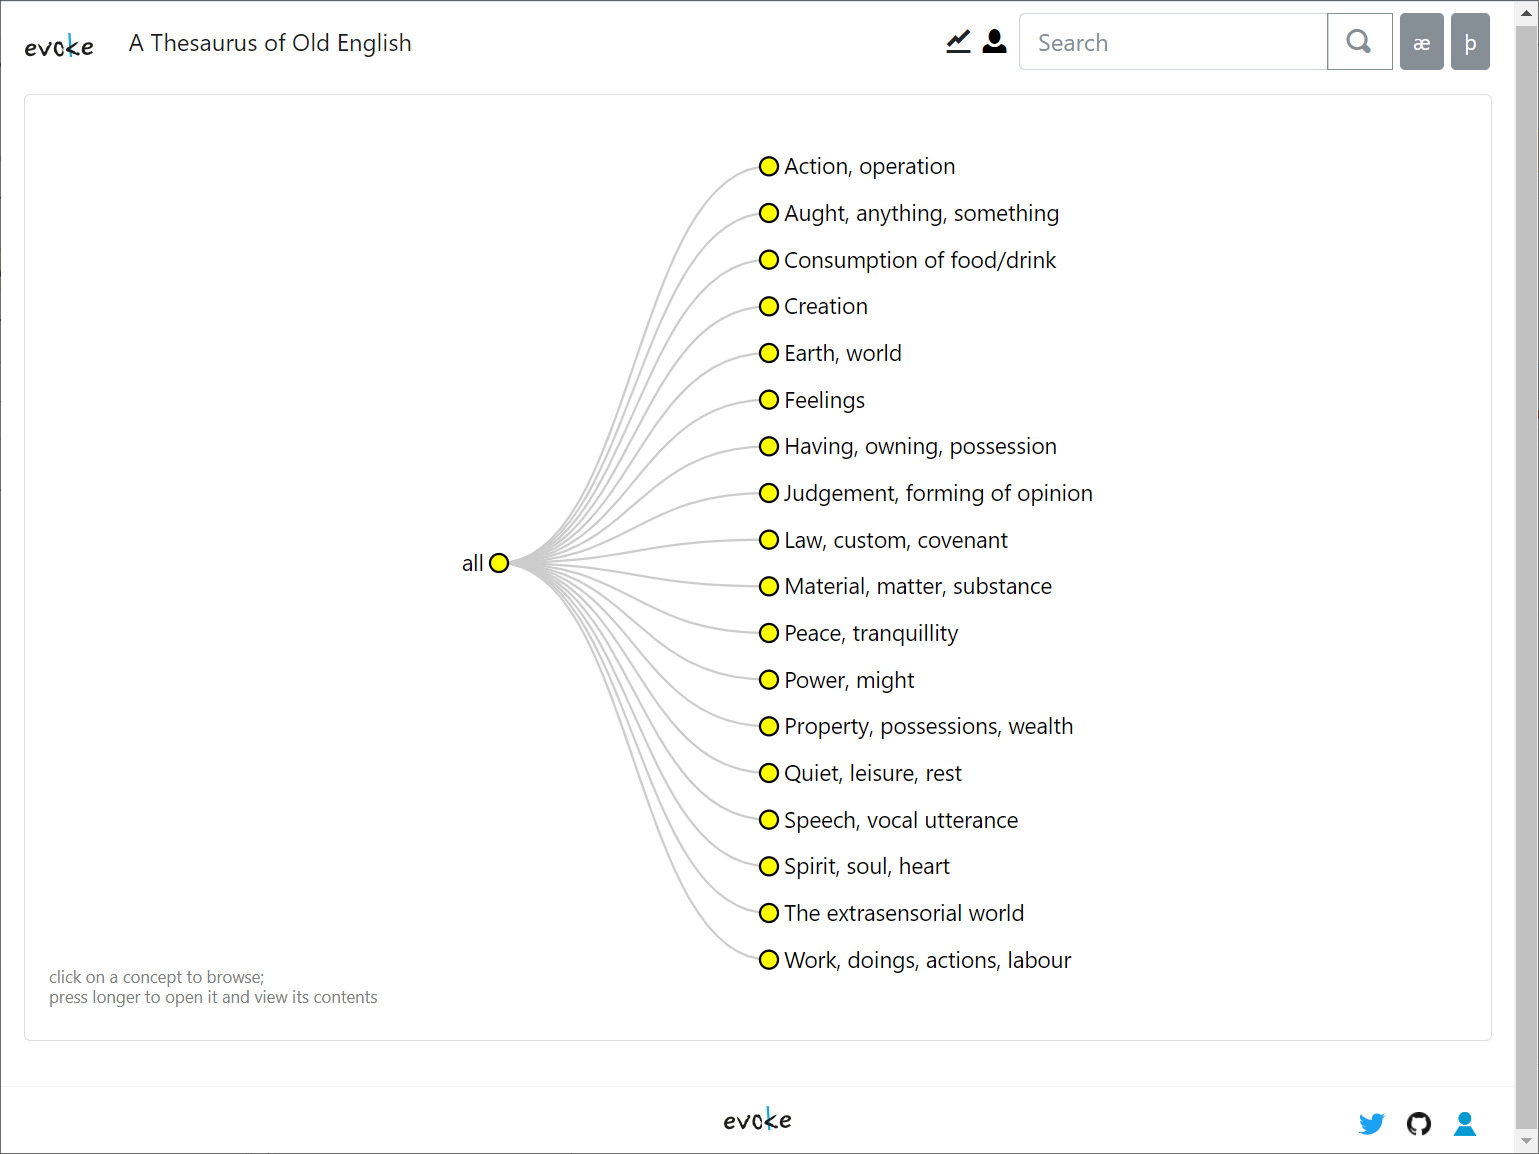
\includegraphics{Stolk2021a/fig/Fig2.png}
	}
	\caption[]{\label{fig:Stolk2021a:Fig2} Navigating the top of the semantic hierarchy of A Thesaurus of Old English.}
\end{figure}

\begin{figure}[htbp]
	\resizebox{\textwidth}{!}{
		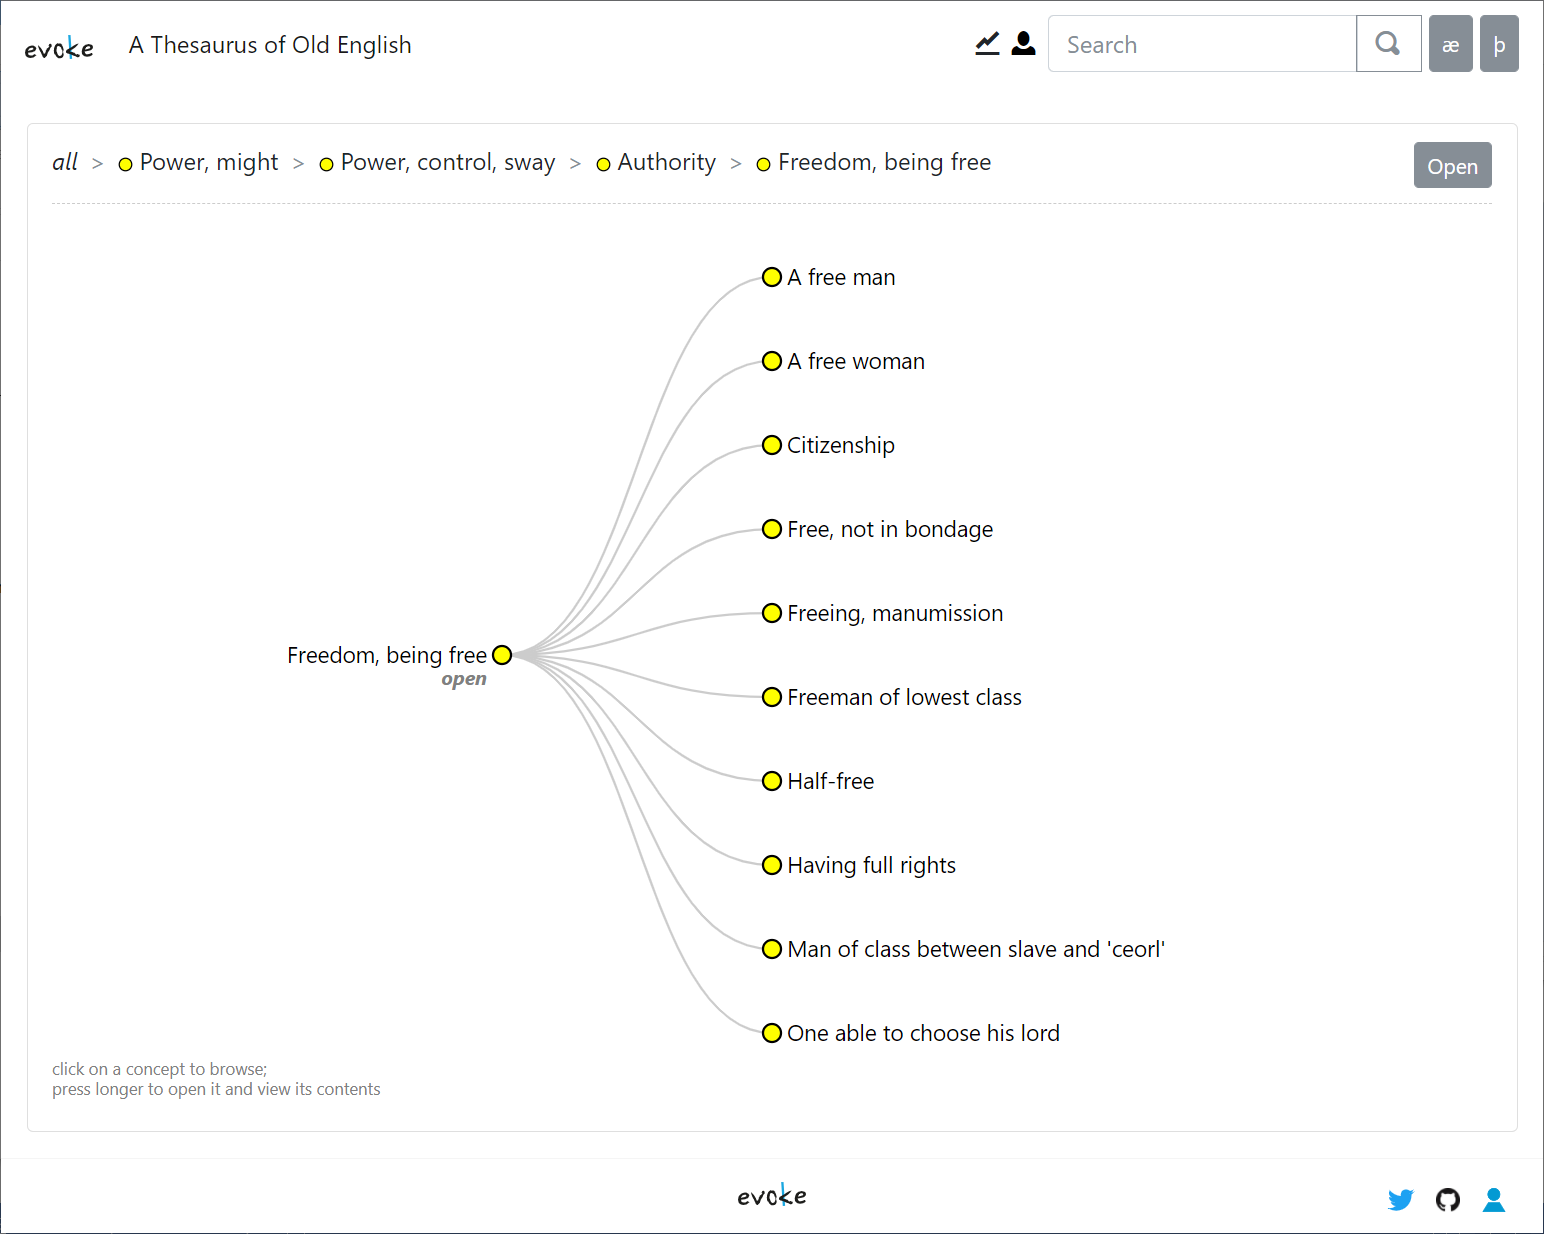
\includegraphics{Stolk2021a/fig/Fig3.png}
	}
	\caption[]{\label{fig:Stolk2021a:Fig3} Navigating the concept “Freedom, being free” of A Thesaurus of Old English.}
\end{figure}

\subsubsection{Searching for Content}
The search engine of Evoke offers the second manner to approach thesaurus content, accessed through a search box in the navigation bar. This component performs searches for semantic concepts, words, word senses, and any other elements (e.g., labels) based on an entered string. Support for wildcard searches is in place: a question mark (?) allows for any character to occupy that position of the query; an asterisk (*) allows for any number of characters to exist at that position. Thus, searching for scip* in A Thesaurus of Old English will result in a number of compound words that start with the element meaning “ship” (see Fig. 4), including the nouns scipāc ‘oak for shipbuilding’ and scipgyld ‘ship-tax’. Wild card searches enable a whole range of research avenues, including identifying Old English kennings — i.e., poetic compounds such as sǣwudu ‘ship, lit. seawood’ — and for looking into the productivity of affixes (e.g., the suffix -lēas ‘-less’ with adjectives).

Search results in Evoke indicate the type of each find: semantic concepts are clearly marked and distinguished from, for instance, lexical items or labels. To illustrate, the dark grey bar in Fig. 4 acts as heading for the results underneath, all of which are senses. Word senses that belong to the same dictionary entry are grouped together, allowing users to select the word as well as one of its specific senses for viewing. For each lexical item, the lemma is preceded by its part of speech (e.g., “noun”) and followed by any labels that are applicable (e.g., “poetry”). As the meanings of word senses are indicated by their location in the semantic hierarchy, word senses in the search results are shown along with the semantic concept that express their meaning (e.g., ‘A voyage’ for sciplād). This presentation enables users to distinguish different senses of the same word from one another.

\begin{figure}[htbp]
    \centering
	\resizebox{0.5\textwidth}{!}{
		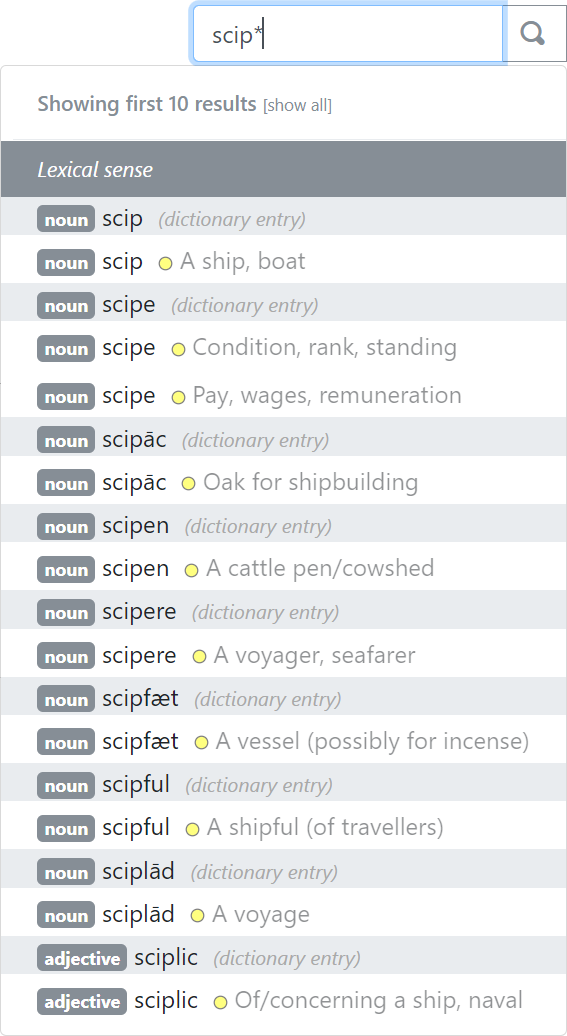
\includegraphics{Stolk2021a/fig/Fig4.png}
	}
	\caption[]{\label{fig:Stolk2021a:Fig4} Search results for scip* in A Thesaurus of Old English.}
\end{figure}


\subsection{Viewing}
On opening a word, word sense, semantic concept, or any other type of element, for viewing, the earlier discussed navigation components are minimized and, instead, an information pane takes centre stage (cf. R2). The pane contains a number of tabs, each offering a distinctive viewpoint on the element in question. The “info” tab presents basic information on the element viewed: its internationalized resource identifier (IRI), name, type (e.g., concept, word sense, etc.), and other properties available (see Fig. 5). For lexical items (i.e., word and word senses) and semantic concepts, the information pane contains a number of additional tabs that incorporate important viewpoints on these Linguistic Linked Data elements specifically.

\begin{figure}[htbp]
	\resizebox{\textwidth}{!}{
		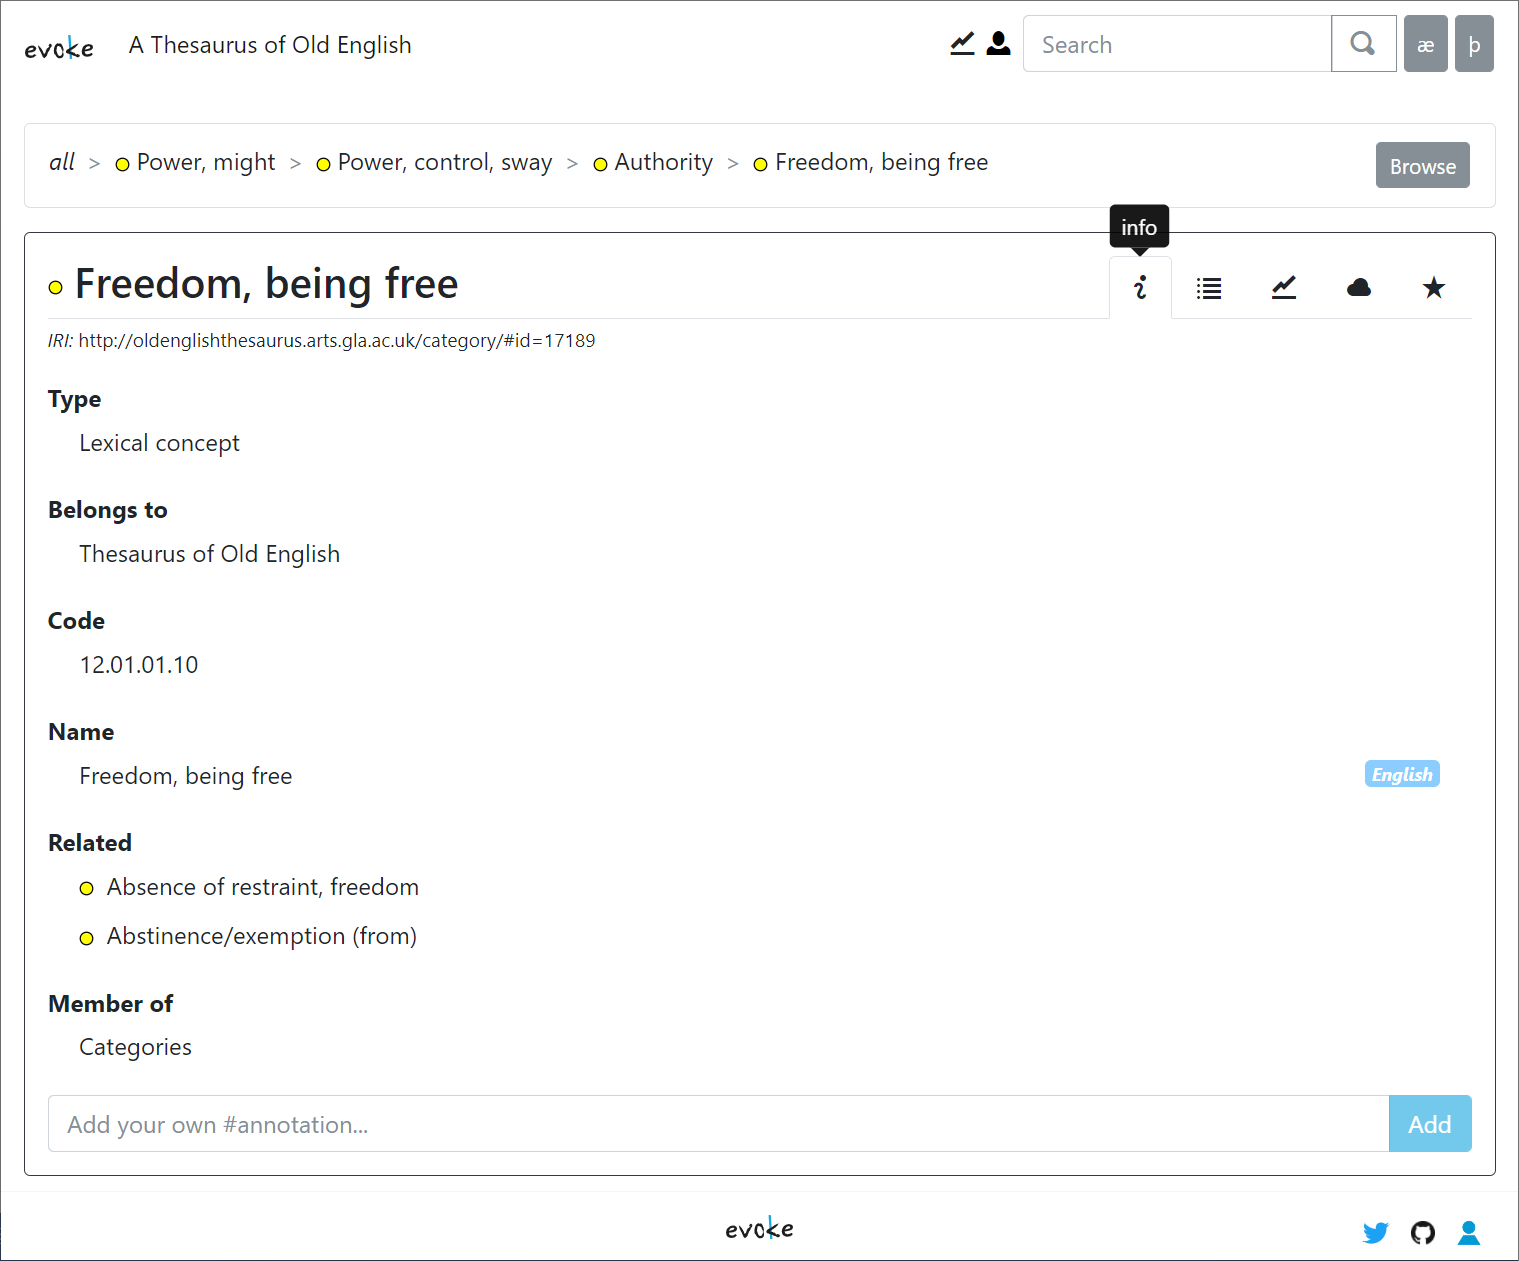
\includegraphics{Stolk2021a/fig/Fig5.png}
	}
	\caption[]{\label{fig:Stolk2021a:Fig5} Information tab of the concept “Freedom, being free” from A Thesaurus of Old English.}
\end{figure}


\subsubsection{Viewing Semantic Concepts}
An information pane on semantic concepts contains four additional tabs: “list”, “statistics”, “wordcloud”, and “associations”. The first of these records the word senses that denote (or lexicalize) the concept that is being viewed. The concept “12.01.01.10 Freedom, being free” in A Thesaurus of Old English, for instance, is denoted by senses attributed to the Old English words frēols and frēot (see Fig. 6). Each word sense listed indicates the part of speech, language (i.e., Old English in A Thesaurus of Old English) and any labels that are applicable either to this particular sense or, more generically, the dictionary entry of the word (e.g., “poetry”). Any of these elements can be clicked for viewing instead of the semantic concept currently shown, utilizing the underlying Linked Data mechanisms.

\begin{figure}[htbp]
	\resizebox{\textwidth}{!}{
		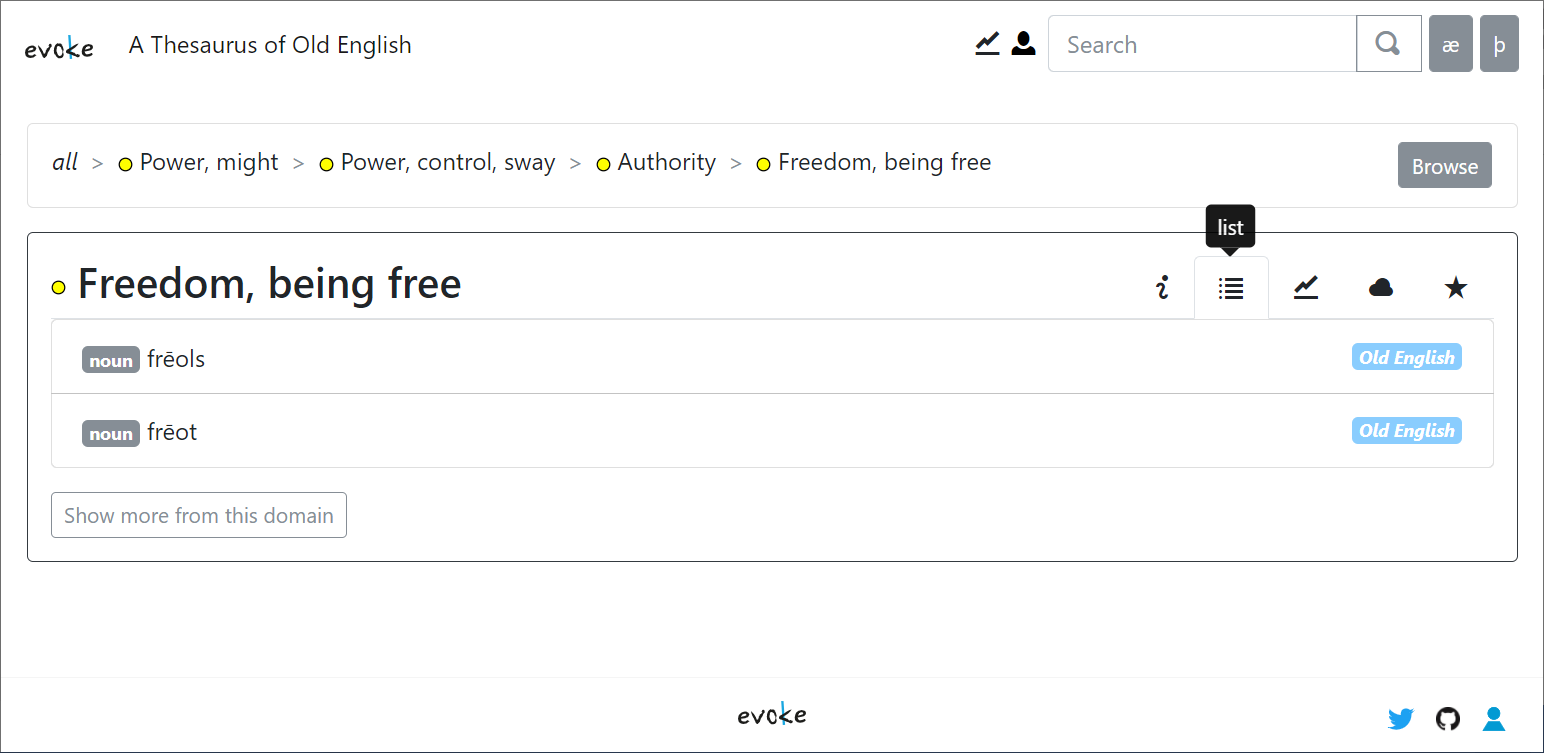
\includegraphics{Stolk2021a/fig/Fig6.png}
	}
	\caption[]{\label{fig:Stolk2021a:Fig6} List tab of the concept “Freedom, being free” from A Thesaurus of Old English.}
\end{figure}


The “statistics” tab provides functionality for analyses and will be covered in section 4.4. The “wordcloud” and “association” tabs present graphical overviews. The former depicts, in a more playful manner, the same words listed on the “list” tab (see Fig. 7). The latter conveys semantic concepts that are evoked by further senses of the words found in this semantic domain, indicating possible connotations captured through polysemy (see Fig. 8).

\begin{figure}[htbp]
	\resizebox{\textwidth}{!}{
		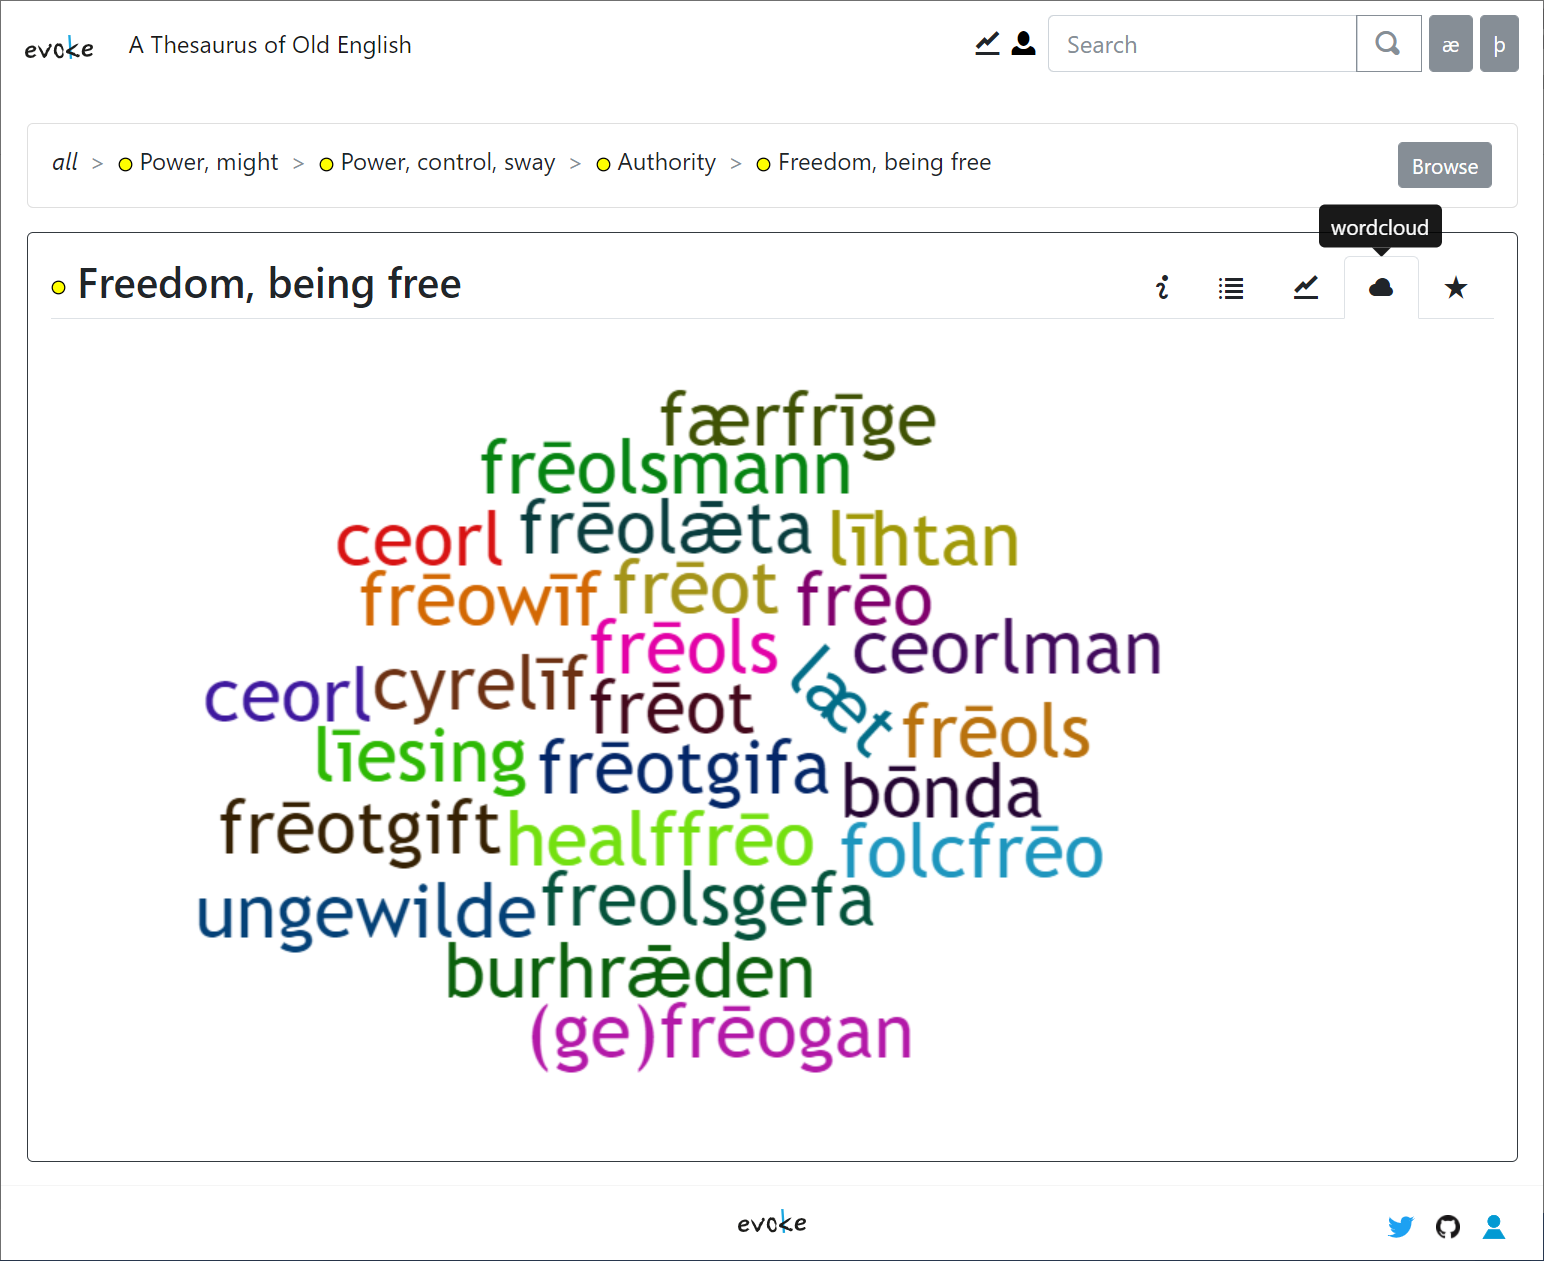
\includegraphics{Stolk2021a/fig/Fig7.png}
	}
	\caption[]{\label{fig:Stolk2021a:Fig7} Wordcloud tab of the concept “Freedom, being free” from A Thesaurus of Old English.}
\end{figure}

\begin{figure}[htbp]
	\resizebox{\textwidth}{!}{
		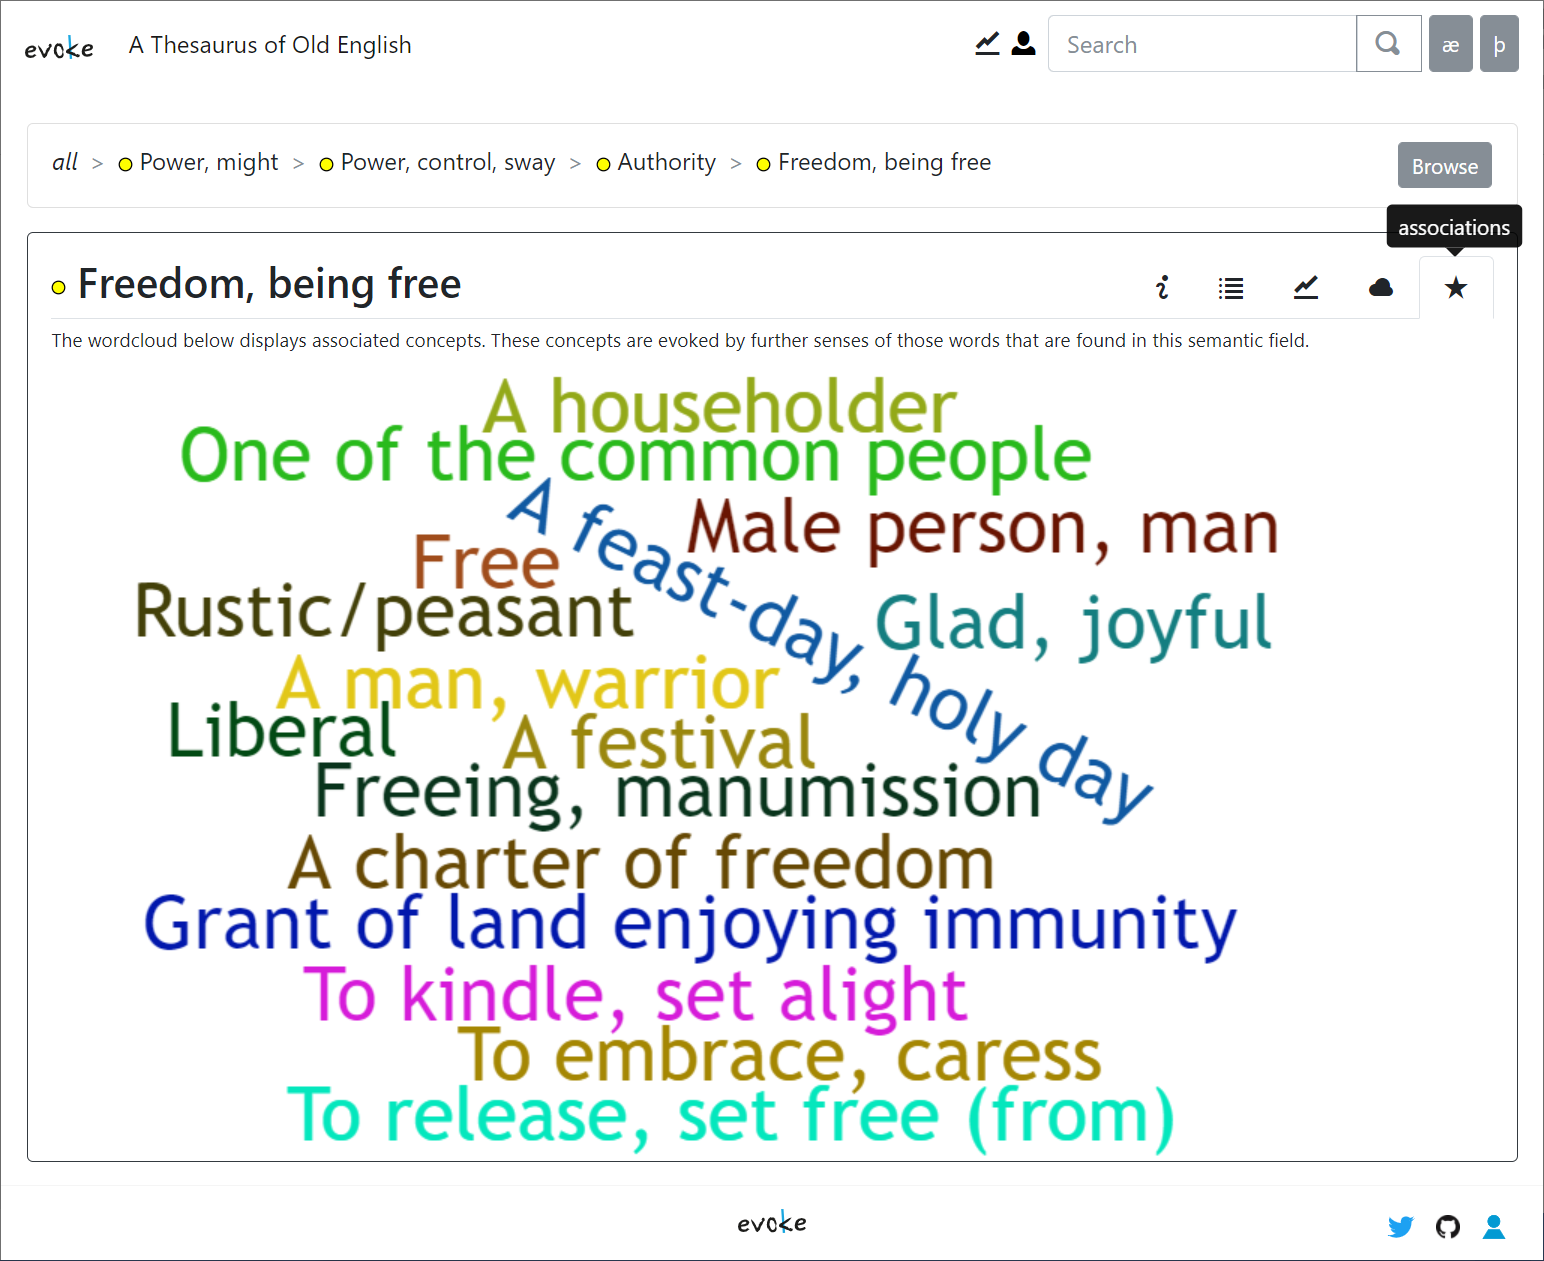
\includegraphics{Stolk2021a/fig/Fig8.png}
	}
	\caption[]{\label{fig:Stolk2021a:Fig8} Associations tab of the concept “Freedom, being free” from A Thesaurus of Old English.}
\end{figure}


\subsubsection{Viewing Lexical Items}
Words and word senses have a similar representation to that of semantic concepts. Fig. 9 contains an information pane for the Old English word þēof in the sense of ‘A robber, thief’. The “info” tab, here, includes synonyms, information on the dictionary entry of the word (in a grey box on the right), and an annotation component (at the bottom, discussed in section 4.3.1). The “list” tab for these items indicates the various polysemous senses available for this word and their place in the semantic hierarchy of the thesaurus. The “wordcloud” tab, again, depicts these listed items in a cloud of words, and can be considered a narrower view of the “associations” tab for semantic concepts — here restricted to a single word rather than all those found in a given semantic domain.

\begin{figure}[htbp]
	\resizebox{\textwidth}{!}{
		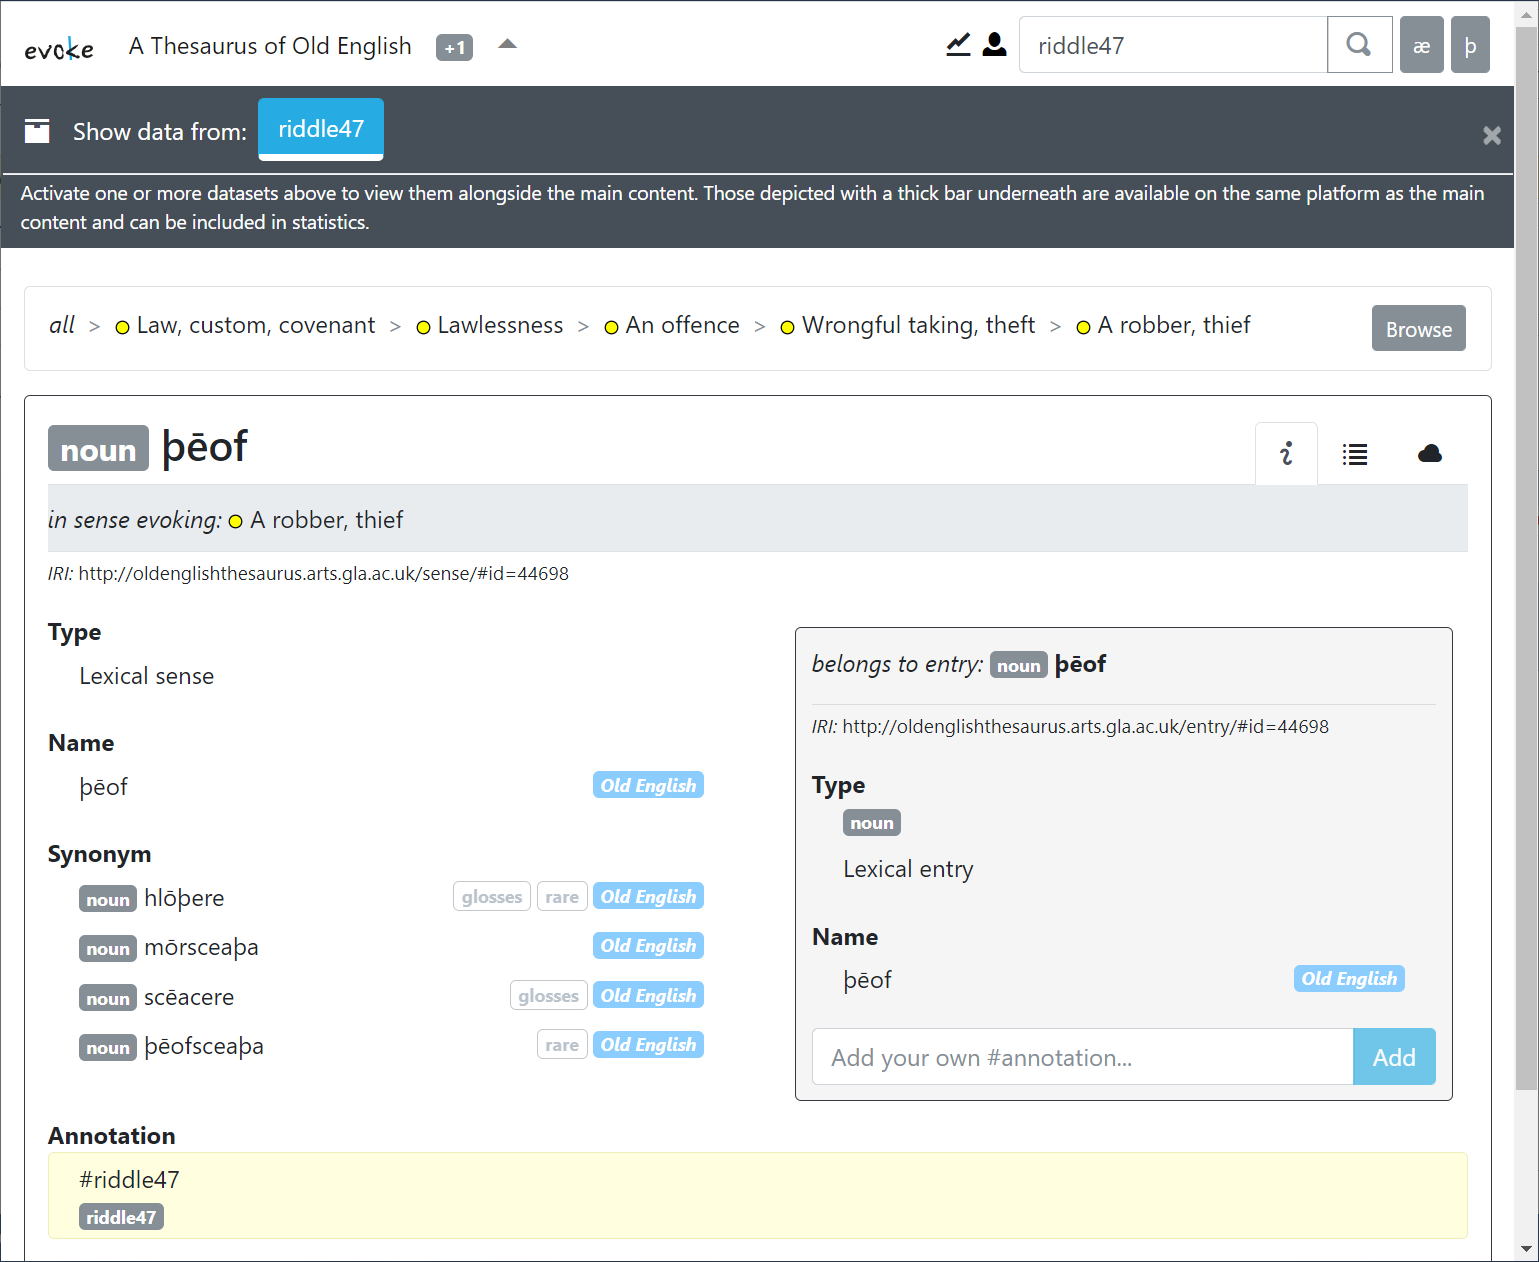
\includegraphics{Stolk2021a/fig/Fig9.png}
	}
	\caption[]{\label{fig:Stolk2021a:Fig9} A sense of the word þēof as described in two datasets (i.e., TOE and riddle47, see top of image).}
\end{figure}

\subsection{Extending}
One of the main requirements for Evoke has been to allow users to extend thesaurus content, thereby adding salient information (cf. R3). Offering such functionality has been done in various shapes before, but tends to require user accounts, online hosting, moderation of user content, and, possibly, users first obtaining a license for full access to the original dictionary data instead of being able to directly engage with the content at hand (cf. AR3). Evoke takes a different approach, utilizing Linked Data in order to bring together thesaurus content and user content. Users can extend content made available in Evoke in two ways: (1) annotating and (2) linking data.

\subsubsection{Annotating}
Users of Evoke can annotate content and add their own labels, allowing them to mark words, or their senses, as being noteworthy in a given manner. A given word can, for instance, be labelled poetic if its use is mostly restricted to poetry. Further usage features that can be marked though such a system of tags or labels include those based on time (diachronic), place (diatopic), formality (diaphasic), and frequency (diafrequential) (Hausmann, 1989: 651-652). Marking words in this manner is known in lexicography as diasystematic labelling (Hartmann and James, 1998). Labels are useful beyond recording usage features, however. Indications of occurrences in a specific text or use by a certain author can facilitate systematic analyses of the vocabulary employed within this context. See research done by Thijs Porck and by Amos van Baalen, part of this special issue, which showcase the application of such textual and authorial labels.

The annotation component is presented on information tabs of lexical elements (see Fig. 9). Although typically used for annotating words and word senses, the component is not limited to use within that scope and could be used for semantic concepts or indeed any other kind of element. The use of the hashtag symbol (\#) in an annotation results in the creation of a corresponding label (e.g., ‘riddle47’ in Fig. 10). Unlike in many existing systems, annotations and labels created in this manner are stored not online in a database but, instead, in the user’s Internet browser.  Additions and remarks belonging to the user can thus be shown and navigated, but are not disseminated or shared from the outset. In practice, this kind of use of browser storage for annotating can be likened to the practice of scribbling in the margins of one’s own printed copy of a dictionary: the original resource (i.e., the thesaurus available for viewing online) is not affected, but only the copy of that resource displayed to the user. In effect, this leads to the creation of a personal copy — one that can be offered without users needing their own user account (cf. AR2).

Users of Evoke are provided full control over their own data. They can download a backup of their annotations and labels in the form of a file, subsequently choose to share these with a select group (e.g., via file sharing or other means), reinsert content in the browser storage, or publish it online for a wider audience to access alongside the thesaurus. As the created backups do not contain the original thesaurus data, but merely the user’s own annotations that reference the identifiers (or IRIs) of the original thesaurus content, users will not breach any license in place that restrains them from downloading the original dictionary data (cf. AR3). Users simply do not download that data; only their own. Thus, mechanisms offered by Linked Data facilitate in negotiating the interests of both users and publishers.

\begin{figure}[htbp]
	\resizebox{\textwidth}{!}{
		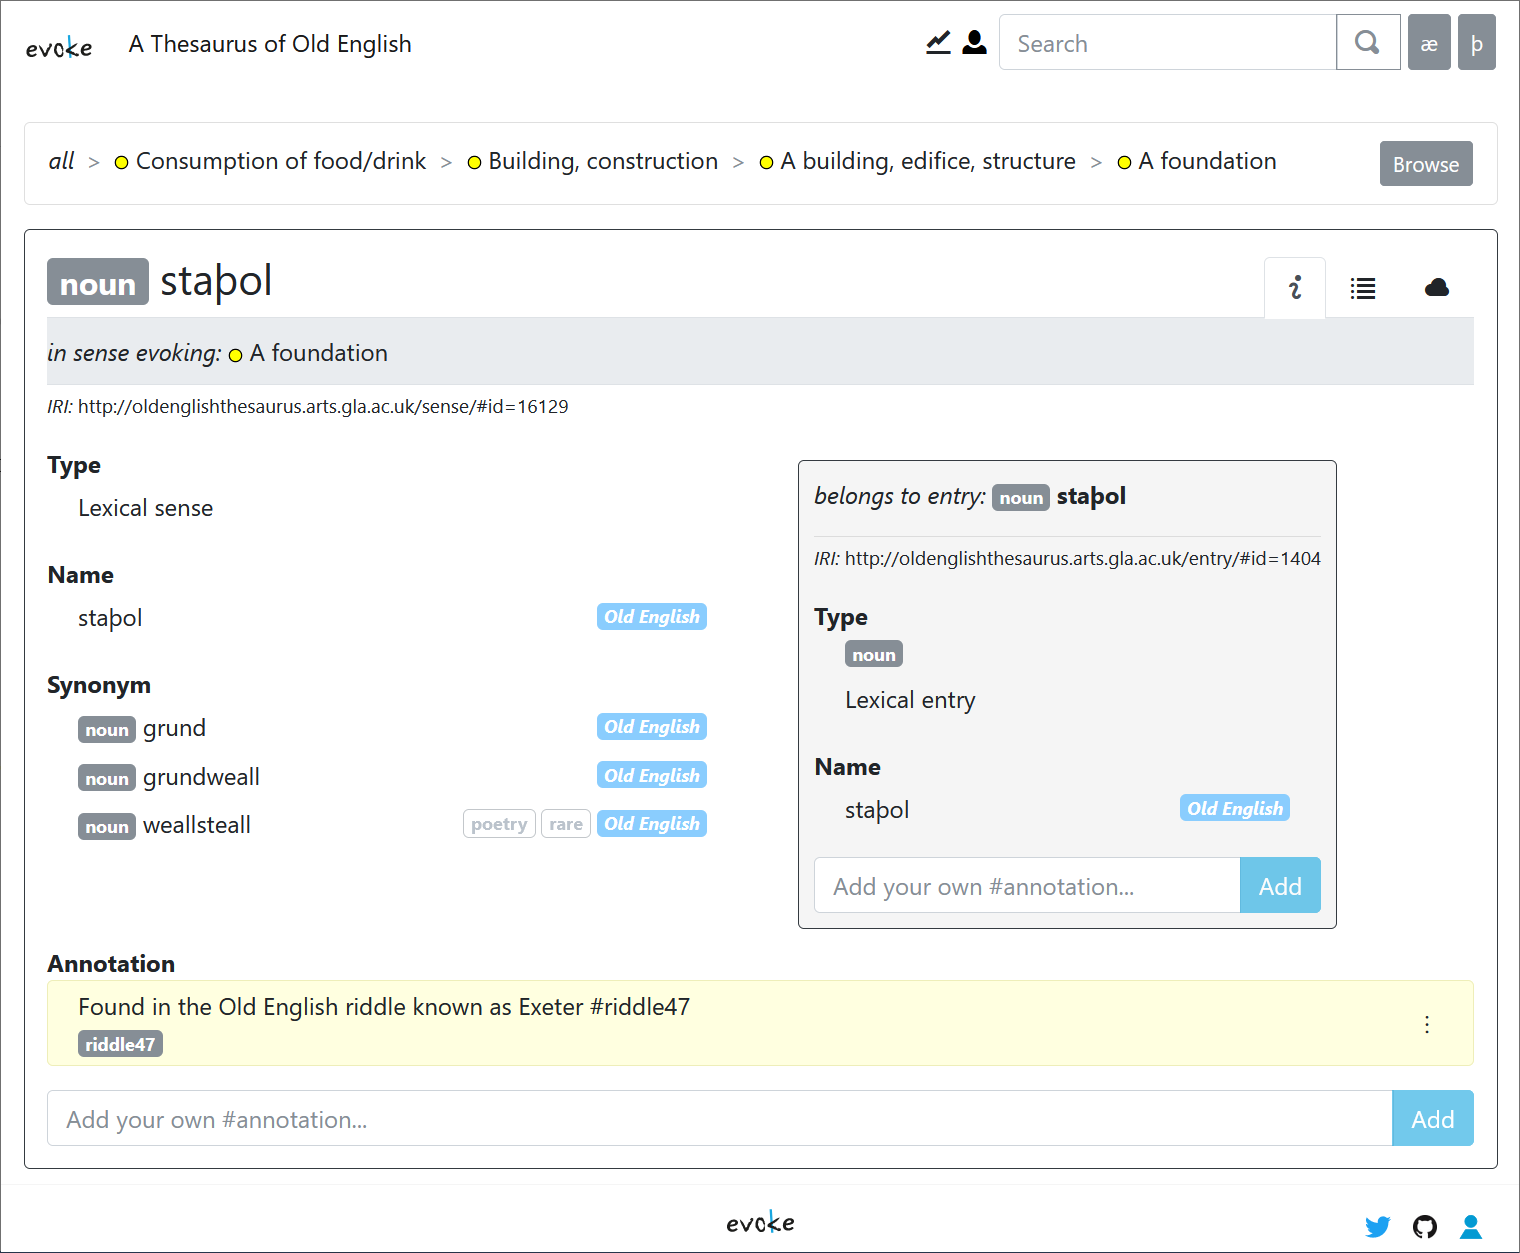
\includegraphics{Stolk2021a/fig/Fig10.png}
	}
	\caption[]{\label{fig:Stolk2021a:Fig10} An annotation in Evoke (bottom) on the Old English staþol in the sense of ‘A foundation’.}
\end{figure}

\subsubsection{Linking Data}
Software other than Evoke can be employed, too, in order to provide additional information on words, word senses, and semantic concepts. The need to facilitate further software to work with and extend existing thesaurus data stems from the fact that some tooling is more suited for a given task (or for a certain audience) than other tooling.  Lexicographers may well prefer one piece of software whereas linguists or philologists may turn to another. The use of Linguistic Linked Data, in which content is identified by means of IRIs, offers the possibility to link linguistic content maintained elsewhere by adding references to these internationalized resource identifiers. Indeed, multiple research projects have adopted this approach. Two of the tools that have been used for this purpose, alongside Evoke, are described below. Publications on the research in which these tools have been used are part of this special issue. Further tooling to create and maintain Linguistic Linked Data is actively being developed (e.g., VocBench 3; see Stellato et al., 2020).

In his research project to create textual thesauri of the Old English poems Beowulf and Andreas, as well as the prose Old English Martyrology, Thijs Porck has employed an alignment tool that was specifically created for connecting data from glossaries of Old English texts to the dataset of A Thesaurus of Old English, already available in Evoke. The tool reads in a glossary of a text edition (in PDF format), extracts information on the words that occur in that Old English text and presents that information in a table. Each table row offers the user the means to search for, match, and link related content (in this case, words) from A Thesaurus of Old English and to annotate these finds with additional remarks or labels (see Fig. 11). Indeed, search results in Evoke can be dragged and dropped in other applications, using the mouse cursor, to create a link.  The alignment thus created can be exported and/or published in the Linked Data format in order to view the results alongside A Thesaurus of Old English in Evoke.

\begin{figure}[htbp]
	\resizebox{\textwidth}{!}{
		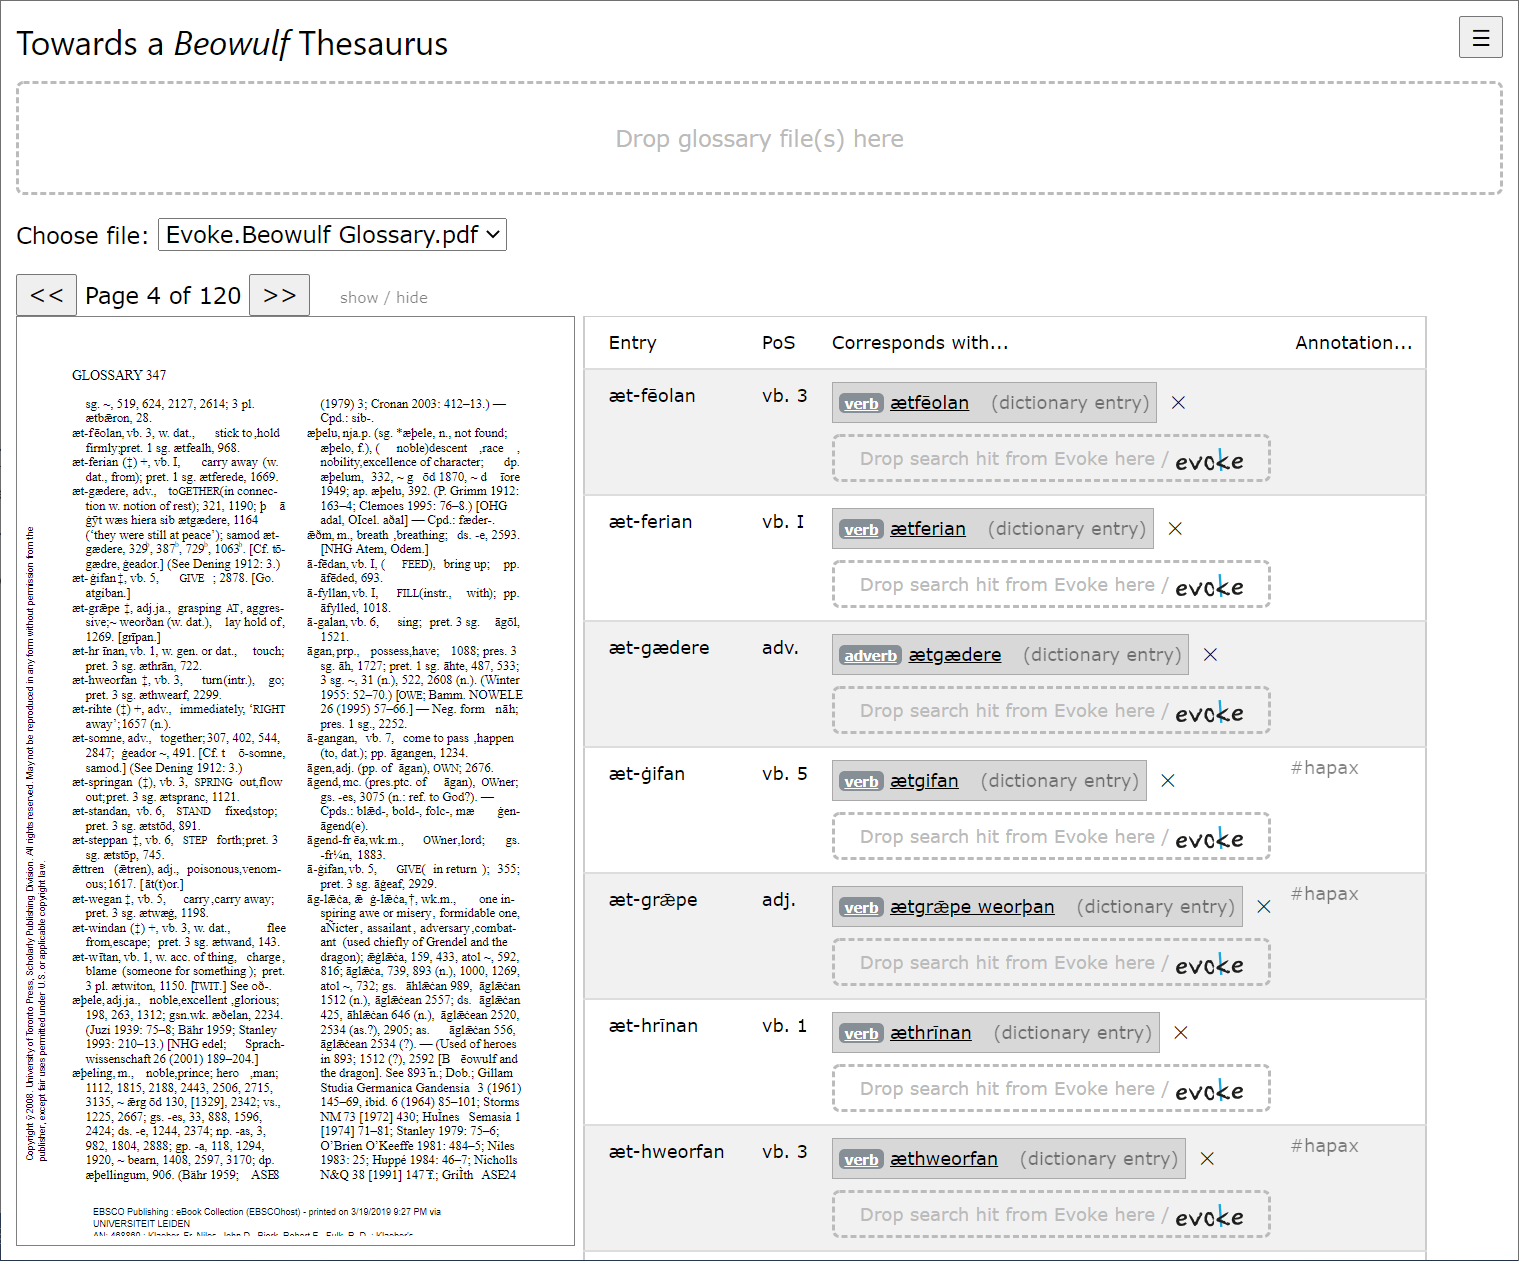
\includegraphics{Stolk2021a/fig/Fig11.png}
	}
	\caption[]{\label{fig:Stolk2021a:Fig11} Alignment tool used for the Old English text Beowulf.}
\end{figure}

In research by Rita van de Poel and Sander Stolk, dictionary data on Old Frisian is linked to A Thesaurus of Old English. A spreadsheet has been used to store information on Old Frisian words and to categorize their senses according to the semantic hierarchy found in the thesaurus (Fig. 12). Each row in the spreadsheet contains information on the sense of an Old Frisian word, which includes the identifier of the word sense (column A), dictionary entry (B), headword (D), language tag (E; here ‘ofs’ for Old Frisian), but also the identifier of semantic concepts that best express their meaning (F). The latter are either IRIs of semantic concepts found in A Thesaurus of Old English or numbers that refer to newly coined ones specific to Old Frisian. In this project, information from the spreadsheet has been transformed to Linguistic Linked Data through the open-source tool OpenRefine along with its RDF plugin. 

\begin{figure}[htbp]
    \framebox[\textwidth]{
	    \resizebox{\textwidth}{!}{
		    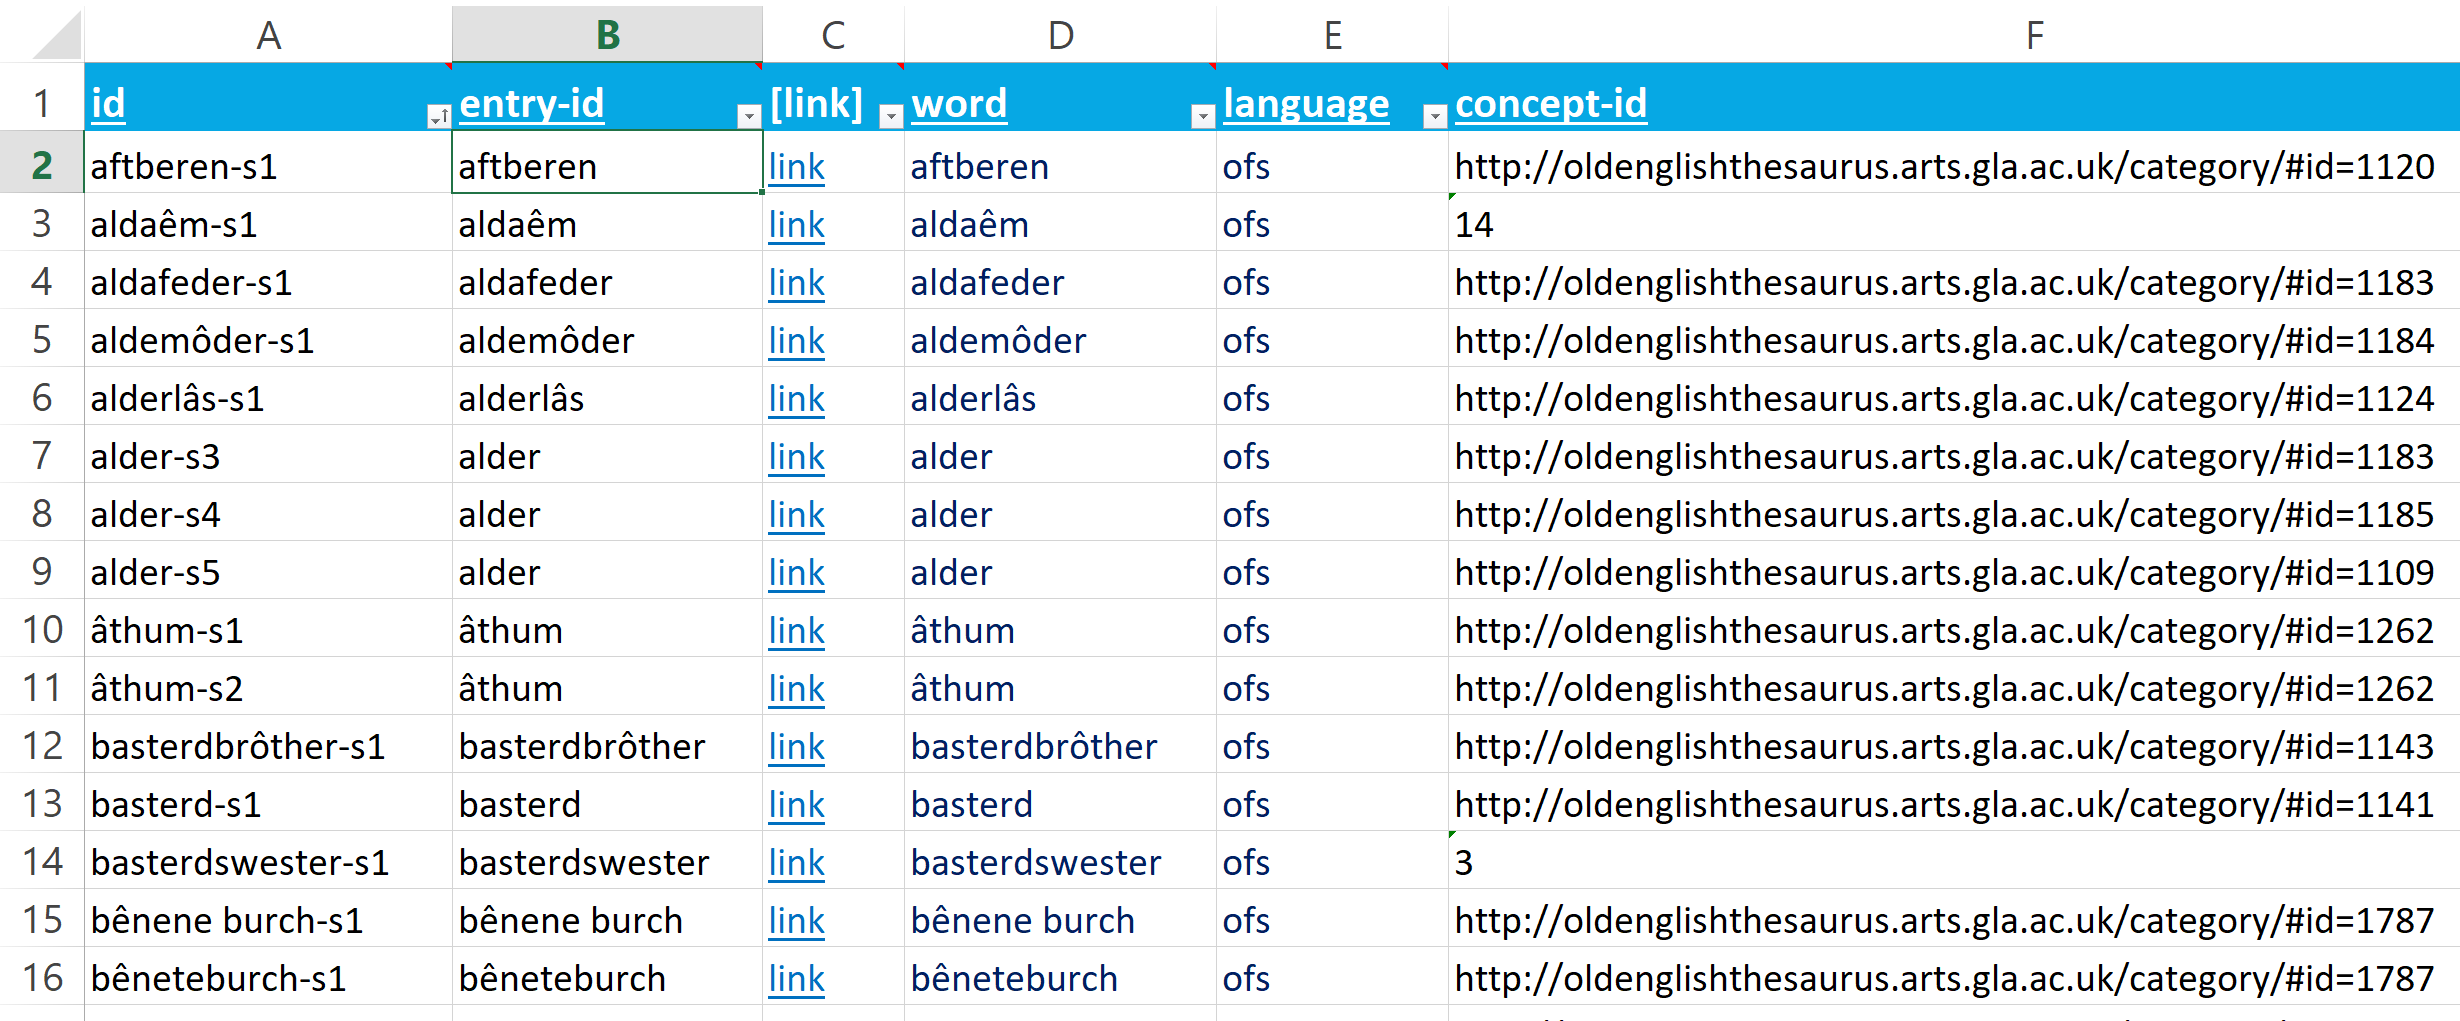
\includegraphics{Stolk2021a/fig/Fig12.png}
	    }
	}
	\caption[]{\label{fig:Stolk2021a:Fig12} Excel spreadsheet used for dictionary data on Old Frisian.}
\end{figure}

\subsection{Analysing}
Thesauri are valuable in analysing the vocabulary of a language community. Scholars have made use of these lexicographic works to investigate a range of aspects encoded in the lexicon: cultural elaboration, semantic domains and their cultural connotations, stylistic preferences of authors or in certain texts, and the use and development of metaphors (e.g., Spevack, 1993; Crystal, 2014; Anderson, Bramwell, and Hough, 2016; Porck, 2016: 59-71, 239-294; Diller, 2017).  Functionality to perform such analyses is therefore valued greatly for research based on thesaurus content. A key requirement for Evoke in opening up thesauri, then, has been to allow users to perform statistical analyses (cf. R4). The analyses should work on the original thesaurus content but, with the ability of users to extend the thesaurus with their own information, also on additional content created by users. This section treats two manners in which users of the Evoke interface can perform analyses: (1) viewing default analyses and (2) building custom queries.  

\subsubsection{Viewing Default Analyses}
Analyses of words in semantic domains are a common use of thesauri. Indeed, in her review of A Shakespeare Thesaurus, Christian Kay mentions that a simple count of word senses under a category is sorely lacking in that lexicographic work (Kay, 1996: 73). Such counts indicate the degree of lexicalization, also known as cultural elaboration, of semantic concepts (Wierzbicka, 1997: 10-11). The underlying hypothesis for the importance of these figures is that domains that are important in a culture are heavily encoded in the language of that community, providing its speakers with a multitude of nuances to discuss the subject. This statistic is, for thesaurus content in a digital environment, relatively straightforward to obtain through queries. Even so, many thesauri — both paper and electronic editions — do not include these rudimentary statistics in their presentations.  

The web application Evoke presents a small set of basic, default analyses under the statistics tab of semantic concepts. Fig. 13 illustrates these analyses for the concept “12.01.01.10 Freedom, being free” of A Thesaurus of Old English. Three charts are shown on this tab. The first is a bar chart that indicates the degree of lexicalization. The viewed concept has 2 words specifically in the sense of “freedom, being free” and 28 further words in a sense that is more specific in meaning (i.e., positioned at subordinate concepts in this branch of the semantic hierarchy). 

The second chart is a pie chart that indicates the distribution of word senses in this domain — including senses positioned lower down the hierarchy — over parts of speech. The chart in Fig. 13 indicates that most words in this domain are nouns (70\%) with adjectives and verbs making up the remainder. As Jan Anward points out, words in a part of speech not only share grammatical properties, but tend to belong to the same semantic category, too (Anward, 2006). Nouns, he argues, denote entities, whereas verbs denote events. Linguists who analyse a semantic domain tend to discuss the parts of speech for the lexis involved or concentrate on a single part of speech.  Providing statistics on the distribution of parts of speech is therefore warranted for users of Evoke. 

The third and last analysis provided by default is the distribution of word senses over the various direct subdomains of the current semantic concept. In other words, this analysis contrasts the various branches from this point in the semantic hierarchy. To illustrate, the chart presented in Fig. 13 conveys that there are twice as many words available to express ‘Freedom, being free: A free man’ than ‘Freedom, being free: A free woman’. Hovering over these slices with the mouse cursor presents their absolute counts (in this case, 4 and 2 respectively) instead of their percentages. In contrasting related domains such as these, users are able to analyse their relative degree of lexicalization and therefore supposed dominance or importance in the language community. The larger the semantic domains analysed, the more valuable it will be for researchers to have these statistics automatically generated as opposed to calculating them manually. In A Thesaurus of Old English, for instance, 1,348 word senses evoke the concept “13.02 War”, whereas the nine co-ordinate domains for peace encompass a mere 119 word senses. A cog wheel shown next to the pie charts allows users to customize these charts by hiding certain slices. Disposing of “13.02 War” thus, visually, would allow one to foreground “peace” and the nuances between the nine co-ordinate domains that deal with this notion.

\begin{figure}[htbp]
	\resizebox{\textwidth}{!}{
		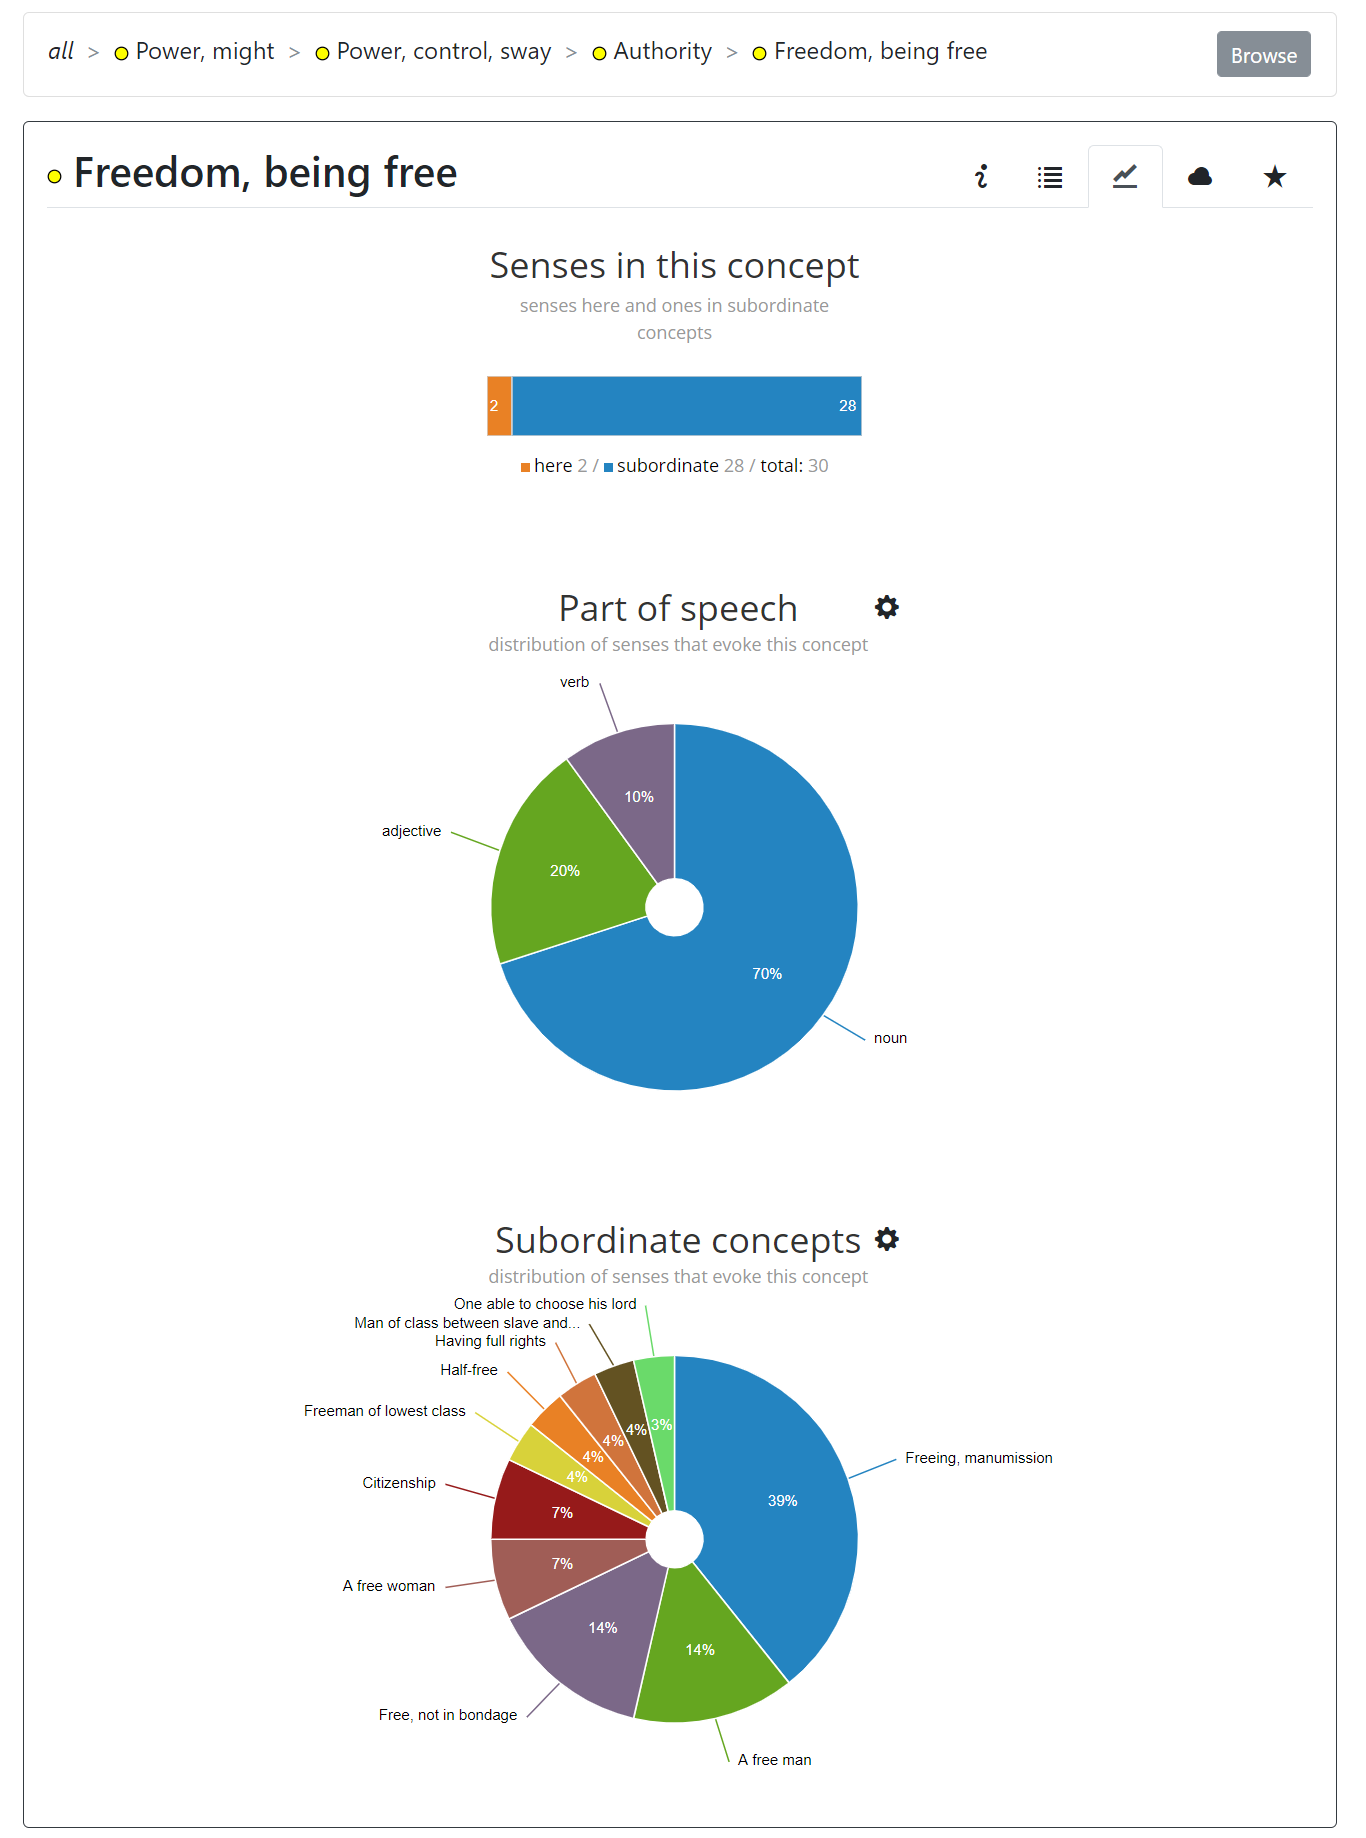
\includegraphics{Stolk2021a/fig/Fig13.png}
	}
	\caption[]{\label{fig:Stolk2021a:Fig13} Default statistics as shown in Evoke for the semantic concept “Freedom, being free”.}
\end{figure}

\subsubsection{Building Custom Queries}
On the analysis page of Evoke, accessible by means of the graph icon in the navigation bar, the interface presents users with a way to build custom queries and perform analyses (see Fig. 14. Users can indicate which items are of interest by selecting features of words or words in a specific sense (called “lexical entries” and “lexical senses” respectively). Features of these items can be selected afterwards: a label, a part of speech, and, in the case where multiple are present, a language. Although a selection can include only one part of speech and one language, it may contain multiple labels to combine features of interest (e.g., “poetry” and “rare” for rarely occurring items found in poetic texts). Possible values for a given feature are presented through a dropdown list. Each option in the list is presented as text.  

\begin{figure}[htbp]
	\resizebox{\textwidth}{!}{
		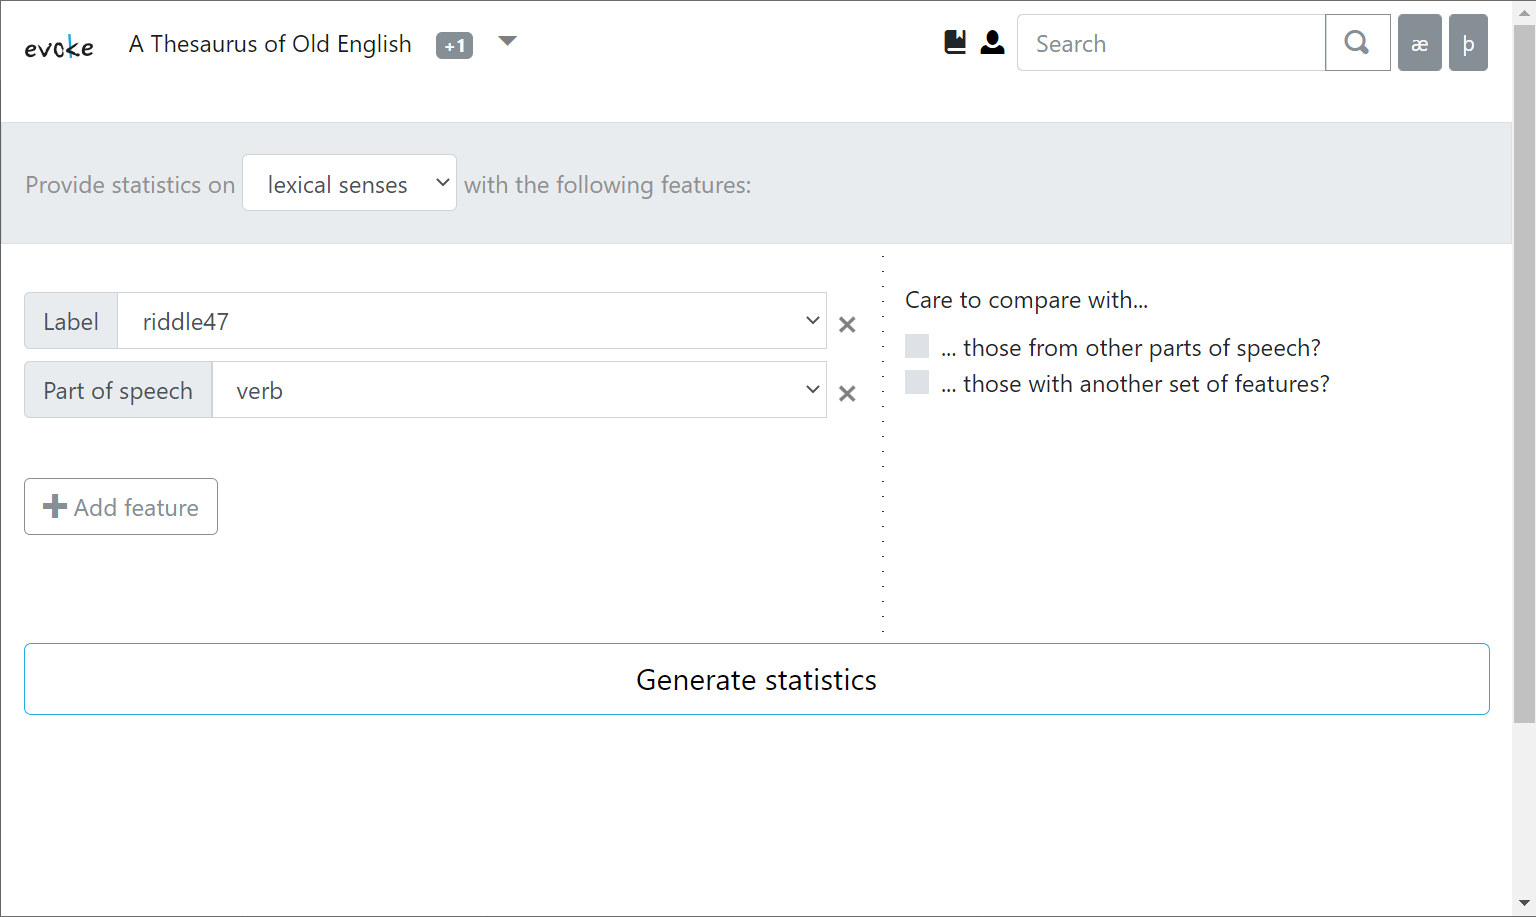
\includegraphics{Stolk2021a/fig/Fig14.png}
	}
	\caption[]{\label{fig:Stolk2021a:Fig14} The form that allows users to select their features of interest in the statistics section.}
\end{figure}

Once one or more features have been selected for analysis, users can opt to compare their selection with items from other languages (if any are available in the data analysed), with other parts of speech, or with another set of features they are interested in. The default choice in analyses is to contrast items of interest with all other items of that kind. Thus, a selection of lexical entries with the labels “poetry” and “rare” would be contrasted with all known lexical entries, regardless of their features. Once a user has formulated their query, statistics can be generated and presented. Details on the selection made are stored as part of the URL (as query string arguments), allowing users to share these results by copying the current Web address from their Internet browser.

Analysis results are shown as charts. Each chart presents a distinctive view on the selection made (see Table 1). Together, the charts represent fundamental analyses that take into account the organization of words and word senses in the overarching semantic hierarchy of the thesaurus, thus offering what we term an onomasiological profile of the selection made.

Chart	Description
Item count	This chart shows the number of items in the selection.
Degree of ambiguity	This chart shows the number of lexical entries based on their sense count, also known as the degree of polysemy. (If the selection criteria are based on lexical senses, this chart plots the entries to which they are attributed.)
Degree of synonymy	This chart shows the number of lexical senses based on their synonym count. (If the selection criteria are based on lexical entries, this chart plots the senses attributed to them.)
Distribution: 
categories	This chart shows the distribution of lexical senses over categories, see Fig. 15. (If the selection criteria are based on lexical entries, this chart counts the senses attributed to these entries.)
Distribution: 
tree depth	This chart shows the distribution of lexical senses over the various levels of the taxonomy, see Fig. 16. (If the selection criteria are based on lexical entries, this chart counts the senses attributed to these entries.)
Table 1. Charts available for an onomasiological profile based on a user-specified selection.

Additionally, the visualisation of most charts (i.e., all but the item count) can be customized to suit research needs. Data series shown can, for instance, be enabled or disabled by clicking on their name in the legend. The x-axis of line charts can be zoomed in through clicking and dragging the mouse over the desired range. The y-axis of charts can be altered, by clicking on one of its value labels, to present values as absolute numbers or as percentages indicating the values relative to the cumulative value of the data series. Moreover, charts can include only those items that are (or have) a lexical sense located in a given branch of the thesaurus taxonomy. Selecting one of the categories in the chart covering the distribution of items over categories will allow the user to dive into that branch of the taxonomy. The resulting cropped selection — applied to all charts — is marked through a bar above the charts. Finally, a table containing summary statistics (average, median, and domain and range of the chart) is available through the button ‘show summary’, located in the top right corner.

\begin{figure}[htbp]
	\resizebox{\textwidth}{!}{
		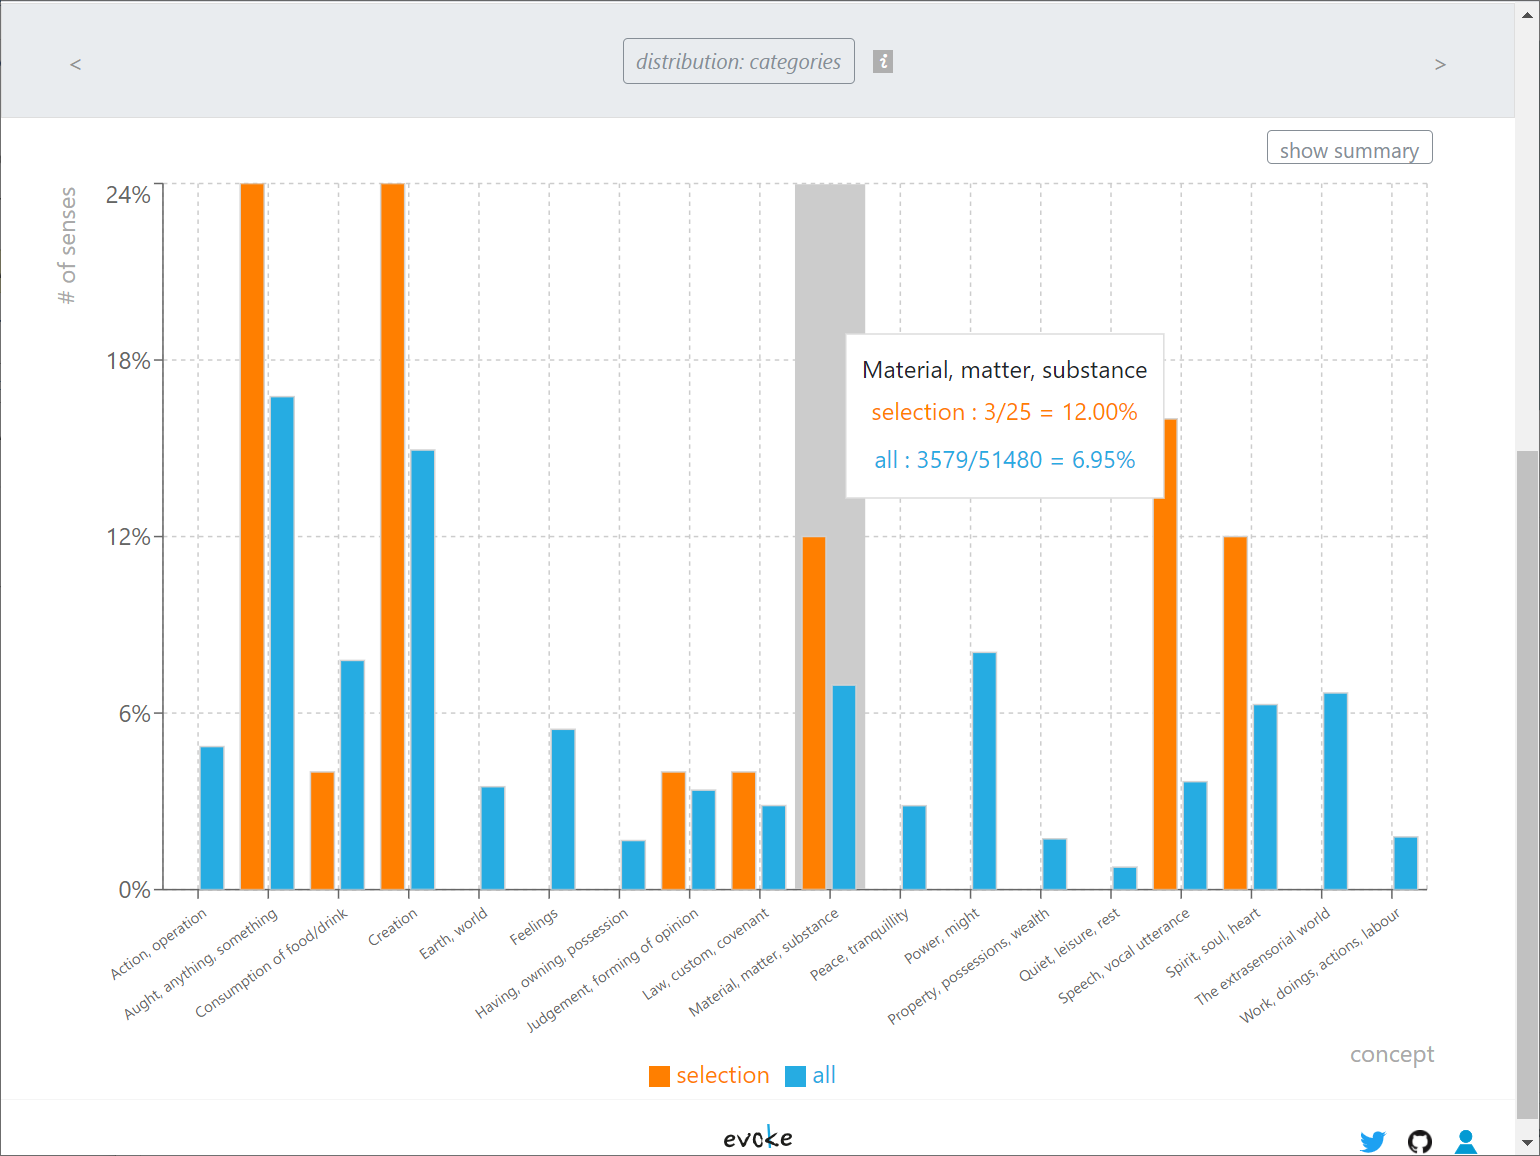
\includegraphics{Stolk2021a/fig/Fig15.png}
	}
	\caption[]{\label{fig:Stolk2021a:Fig15} The distribution over semantic concepts of word senses labelled ‘riddle47’ (orange) versus all senses (blue).}
\end{figure}

\begin{figure}[htbp]
	\resizebox{\textwidth}{!}{
		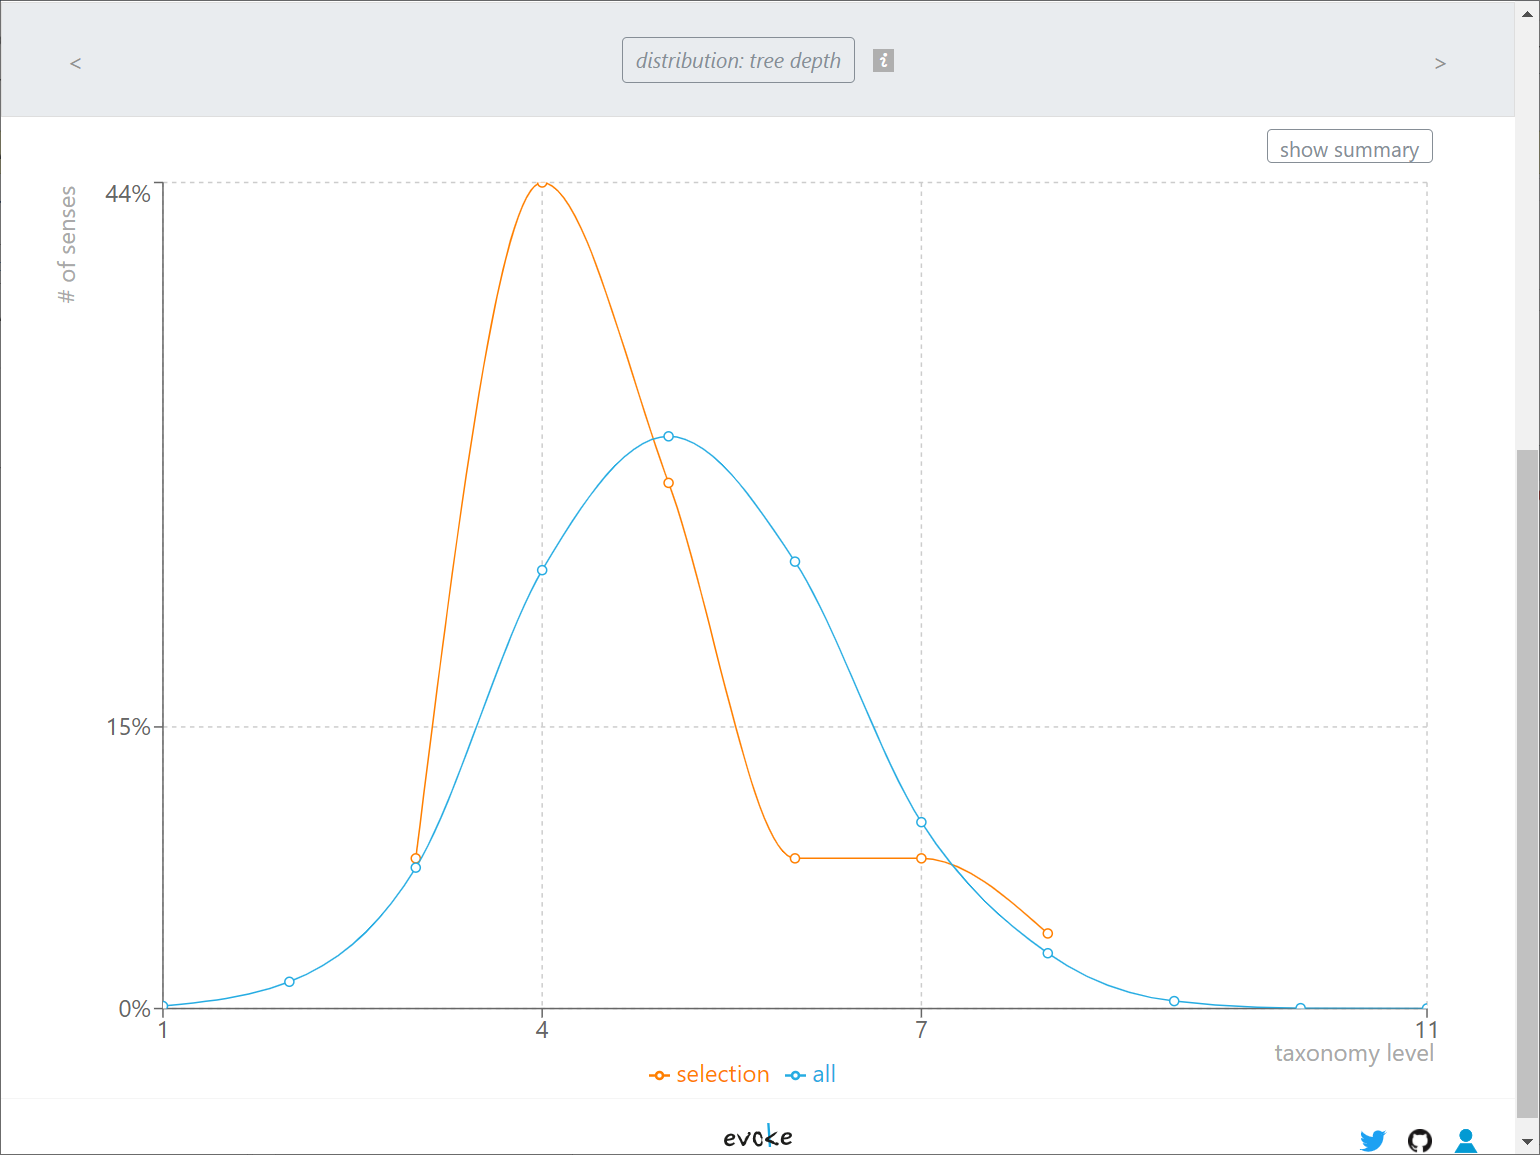
\includegraphics{Stolk2021a/fig/Fig16.png}
	}
	\caption[]{\label{fig:Stolk2021a:Fig16} The distribution over taxonomy depth of word senses labelled ‘riddle47’ (orange) versus all senses (blue).}
\end{figure}

\section{A Thesaurus of Old English as Linguistic Linked Data}

The first lexicographic resource made available in Evoke as Linguistic Linked Data (LLD) is A Thesaurus of Old English (henceforth TOE). This thesaurus captures the lexis of Old English, the early medieval variant of English spoken between roughly 500 and 1100. Upon its first publication in 1995, this resource has been met with high praise, having been called “the most important contribution to Old English studies for years,” since the “comprehensive analysis” that it establishes allows scholars to “investigate what distinctions Anglo-Saxons felt important enough to make in the lexicon” (Görlach, 1998: 398). 

The LLD version of TOE (henceforth TOE-LLD) has been available in Evoke since 2018, based on an extract of the TOE database on May 26th, 2017 that was kindly provided by the University of Glasgow. The majority of the elements within the database were straightforward to translate into Linguistic Linked Data. The Modern English “categories” in TOE, for instance, correspond with “lexical concepts” in LLD; “lexemes”, which have been allocated to TOE categories in the extract of the database, correspond with a LLD “lexical sense” (i.e., a word in a specific sense) that “lexicalizes” a concept.  For details, see Stolk (2019).  One aspect in transforming TOE to TOE-LLD has been altered since that publication and warrants further explanation.

The original database of TOE does not group different senses of a single word under a single entry, a practice typical in dictionaries. Even so, research can benefit from such lexical entries. A case in point is A Beowulf Thesaurus, which marks words used in the Old English text Beowulf (see the contribution by Thijs Porck in this special issue). Marking word senses rather than words, instead, would have constituted an interpretive act which can be likened to translation of the text. Selected senses may not coincide with the author’s original intentions, and would discard some of the ambiguity that the poetic text holds. This interpretive act is one that was avoided in the creation of A Beowulf Thesaurus, but demanded lexical entries to be present in TOE-LLD. Thus, words rather than separate word senses could be marked as occurring in Beowulf. Moreover, distribution flags in TOE “relate only to word forms, not to meanings”.  As a consequence, these flags convey information beyond the level of a lexical sense and can be considered to belong to lexical entries instead, albeit ones implicit in the original database.

In order to enrich TOE-LLD with entries, senses were grouped automatically if they had the following in common: their headwords, their parts of speech, and the distribution flags attributed to them (e.g., “p” for items found only in poetry, “g” for those found only in glosses; see contribution by Jane Roberts in this special issue). Based on these features, “lexical entries” were created in TOE-LLD. As contributors to this special issue point out, the automated detection of entries is by no means perfect: TOE occasionally records separate word forms for a single lemma (e.g., gēardagas and gēardagum), homonyms may be grouped together (e.g., dung meaning “dung, manure” and “dungeon, prison”), and, although rare, distribution flags may not be attributed consistently for different senses of the same lemma (see the contribution by Porck to this special issue). Addressing these issues will require manual verification in order to merge or separate entries that have been created. 

Evoke offers some functionality for interacting with TOE beyond that provided by the existing website of the thesaurus hosted by the University of Glasgow. The original website lacks the means to extend the thesaurus, due partly to licensing concerns. In contrast, Evoke allows for the extension of the thesaurus content by annotating and creating links, which is facilitated by the LLD version of TOE. Not only categories have an IRI in TOE-LLD, as is the case on the original website, but every element is identified by one: from categories to lexical senses and labels. Moreover, Evoke offers the means to perform automated analyses on the information available, based on the semantic hierarchy of the thesaurus, resulting in onomasiological profiles.

\section{Evoke and Old English studies}

To assess the usefulness of Evoke both in research and for education, a research project was formulated with the title ‘Exploring Early Medieval English Eloquence’ (EEMEE). This project has brought together seventeen scholars from universities and lexicographic institutions from across Europe to explore the contents of TOE using Evoke, from a variety of disciplinary perspective, ranging from linguistics to literary-criticism, history, lexicography, and philology. In their explorations, the researchers (and in educational settings, their students) set about viewing other material next to that of TOE, some by linking an already existing source and others by using the annotation system in Evoke. These researchers have been able to access and extend the thesaurus through the use of Evoke, performing advanced analyses, whilst abiding by the license of the lexicographic resource, which restricts them from extracting or downloading substantial portions of the dataset. The results of some of their research projects are included in this special issue.

Novel research done within EEMEE includes analyses of lexis used in specific texts (e.g., Beowulf, see Thijs Porck in this special issue) or used by specific authors (e.g., Ælfric, see Amos van Baalen in this special issue). Their analyses have generated new insights into semantic choices made by Anglo-Saxon authors in individual texts or across an entire oeuvre. The onomasiological profiles thus established may act as semantic fingerprints that can be used in comparative analyses. Other research has focused on metaphors associated with anger and their development through the history of the language (see Khan et al. in this special issue). Lastly, a number of researchers have worked on linking Old Frisian and Old Dutch lexis on kinship with the semantic hierarchy of the thesaurus, which allows us to contrast how many nuances these language communities respectively had, next to those of Old English, in expressing such concepts (see contributions by Rita van de Poel and Sander Stolk; and by Katrien Depuydt and Jesse de Does). All the aforementioned researchers have linked up additional information to the original thesaurus content.

As regards the usefulness of thesauri in education, in the past two years students have used Evoke and TOE to explore aspects of Old English language and culture. At the University of Groningen, Evoke has been used as part of an introductory course to Old English (see the contribution by Kees Dekker in this special issue); students at Leiden University participate in a 2-hour workshop that familiarizes them with digital tools and resources for studying Old English: TOE and Evoke, alongside the DOE and the DOEC.  The learning exercises created at both universities are to be incorporated in the Evoke website. By courtesy of Prof. Carole Hough (University of Glasgow), these exercises will include units from the module Learning with the online Thesaurus of Old English (Hough and Kay, 2017). 

In short, the dataset of TOE has been put to new and innovative use within the field of Old English studies through Evoke. This has allowed the examinations presented in this special issue to provide valuable insights into Old English language and culture. In addition, some of the projects have also led to refinements of the original thesaurus content itself, which were incorporated by the editors of TOE, including the insertion of new words and corrections of distribution flags. An unfortunate side-effect of these very recent, minor improvements of TOE is that, as of writing this article, the lexicographic resource offered on the website by the University of Glasgow is slightly more up-to-date with the current state of Old English lexicography than the TOE-LLD version available in Evoke. Creating a way of automatically synchronizing TOE-LLD with the original TOE database, in order to avoid discrepancies however minor, is therefore desirable and prioritized on the roadmap for future work surrounding Evoke.

\section{Digital Humanities and Onomasiological Research}

Digital approaches for investigating various facets surrounding language, including the structure of vocabularies and diachronic perspectives on language development, are by no means new. Such matters have often been explored, in various branches of computational linguistics, with digital corpora and analytical tools (Sula and Hill, 2019). Onomasiological approaches to language, too, have a long history. Early works in which words and phrases have been arranged thematically, rather than alphabetically, date back as far as Antiquity and possibly further still (Hüllen, 1999: 44). Knowledge catalogued by onomasiological works have had numerous uses: interpretation of texts in foreign languages, selection of words or phrases more suitable in textual composition, and studies of entire semantic fields (Hüllen, 1999).  Since the last century, research programmes have sought to further harness the potential of digital thesauri, whether digitized or born-digital. Automated uses, taking advantage of their digital form, include natural language processing and automated translations.  This section positions Evoke within a number of important developments within the field of Digital Humanities that deals with the study of lexicography and onomasiology.

First and foremost, the efforts surrounding Linguistic Linked Data and software developed for exploring resources expressed in this format constitute an important context for Evoke. These efforts, as Declerck et al. (2020) have observed, play “an increasing role in eLexicography” (5664). The English WordNet, for instance, has recently been ported to this model (McCrae et al., 2020). Moreover, several recent initiatives aim at building and maintaining Linguistic Linked Data resources, including the H2020 projects ELEXIS (2018-22), Prêt-à-LLOD (2019-22) and the COST Action NexusLinguarum (2019-23).  Tooling in these initiatives that work with Linguistic Linked Data focus on creation, discovery, transformation, and linking (Declerck et al., 2020). Examples of such tools include LingHub, which offers discovery of language resources by searching through their metadata (McCrae et al., 2015), and NAISC, used for aligning two RDF datasets.  Unfortunately, most applications currently available for working with Linguistic Linked Data “come with a considerable entry barrier and they address the advanced user of RDF technologies rather than a typical linguist” (Chiarcos et al., 2020). Evoke is amongst the first range of applications that aims to provide a user-friendly interface for such resources and to open them up to a wider audience. Other notable applications that provide user interfaces for Linguistic Linked Data resources are VocBench 3 and LexO (Stellato et al., 2020). Both of these web-based platforms allow users to edit and view Linguistic Linked Data in a user-friendly manner. However, unlike Evoke, they lack functionality to perform onomasiological analyses: their main aim is to manage and publish content collaboratively.

Evoke can also be compared to software capable of working with Linked Data in general or, more specifically, with indexing thesauri expressed in that format, which is more prevalent than that for Linguistic Linked Data. WebProtégé and TopBraid are examples of tools that allow users to edit the graph-like structure of Linked Data through a user interface (Tudorache et al., 2013).  Thesauri adhering to the SKOS vocabulary in Linked Data, which will henceforth be referred to as indexing thesauri, tend to resemble the semantic hierarchy of a lexicographic thesaurus: they identify concepts, possibly arranged in a hierarchy, that are used to index material (e.g., images, documents). PoolParty and Skosmos are instances of web-based tools that allow for editing and documenting indexing thesauri, respectively (Schandl et al., 2010; Suominen et al., 2015). Thesauri represented as Linguistic Linked Data are, not coincidentally, also based on SKOS for their semantic hierarchy (indeed, a ‘lexical concept’ in OntoLex is a specialization of a SKOS ‘concept’) but add additional terminology to capture lexical entries and senses, which are effectively indexed through their evoking and lexicalising of concepts (Stolk, 2019).

Evoke also shares some characteristics with software that offers functionality for extending resources on the Web through Linked Data mechanisms. Such functionality, although not applied specifically to Linguistic Linked Data, is pivotal in notable recent work such as the tool hypothes.is,  used specifically for annotating webpages, and the ecosystem SOLID, which relies on personal RDF data hubs.  Both works use online databases to store information of users, requiring them to login to their account before they can add data. In contrast, Evoke demands no login as user data is stored locally, i.e., in memory of the internet browser, instead. Evoke grants users complete control over their own data and annotations (backup, share, publish), does not demand for that data to be stored online in a centralized manner, and requires no account details before interacting with a resource and extending it. This approach both avoids public comments cluttering webpages of annotated resources and encourages users to engage in open science. 

Lastly, a number of recent research programmes have increased efforts that expand the use of thesauri to other domains. The onomasiological lens that HTE provides, for instance, has been utilized for mapping metaphors throughout the history of the English language (Anderson, Bramwell, and Hough, 2016) and for semantically annotating entire textual corpora for topical analyses (Piao, 2017).  Similarly, the work on Evoke has sought to contribute novel methods to Digital Humanities research for engaging with thesauri. By offering statistical analyses utilizing the semantic hierarchy of these lexicographic resources, and by allowing researchers to link additional information to thesaurus content, Evoke grants new, meaningful insights into a language and the use of its vocabulary in cultural expressions (e.g., individual texts or entire oeuvres). The functionality available offers results that, as a number of researchers point out in this special issue, provides additional knowledge, but may also raise new questions that warrant a closer inspection of the social context (e.g., textual, historical, socio-economic). Evoke, therefore, is firmly rooted in Digital Humanities, and provides the means to explore Humanities-based questions through digital tools that complement, but not supplant, knowledge and expertise of scholars.

\section{Conclusion}

Evoke is one of the first applications that provides a user-friendly interface for working with Linguistic Linked Data resources, opening up TOE to users interested in engaging with its lexicon from an onomasiological perspective. The design of this web application ensures users can view, navigate, extend, and analyse thesaurus content together with relevant, linked datasets. In doing so, they are able to explore the vocabulary of a language community and its relation to their culture. The usefulness of attaching salient information to a lexicographic resource such as TOE is demonstrated by the research presented in this special issue journal. Each contribution showcases how Evoke allows for novel engagement with the Old English lexicon in exploring and extending TOE. 

Future work on Evoke will have two main aims. The first is to improve its functionality for research and education using TOE. Future functionality most frequently requested by researchers is the ability to filter content when navigating and viewing (e.g., based on user-defined labels). This feature would effectively allow users to create specialized subthesauri. Another request is the means to link attestations in corpora to thesauri content, which would permit incorporating frequency analyses in onomasiological profiles. The second main aim for future work on Evoke is to enhance its uptake for research and use beyond Old English studies. Support for additional linguistic resources (including non-English, historical language, multilingual, and sign language datasets), and possibly also indexing thesauri, is considered key for such developments. Moreover, users should be provided with the means to develop their own thesauri instead of working with ones already published and transformed to Linguistic Linked Data. These future developments are planned through collaborative efforts with researchers and language experts from multiple institutes, across national boundaries. 

If the initial work on Evoke is any indication, ventures into Digital Humanities depend on collaboration and creativity of researchers as much as on the digital tools that facilitate novel research queries (or, perhaps, even more so). Since onomasiological investigations rely on the meanings people attribute to symbols (i.e., words and phrases), this human aspect will always remain important in the computer-assisted exploring, extending, and analysing of thesauri.

\section{Acknowledgements} % TODO: unnumbered
This work was supported by the LUCAS Extra Resources Open Call-II Grant 2020, awarded by the Leiden University Centre for the Arts in Society, and the LUCDH Small Grant 2018, awarded by the Leiden University Centre for Digital Humanities. The author would like to thank the researchers and students who – through workshops, courses, and research projects – have used Evoke and provided valuable input for its development.

\section{References} % TODO

Adamska-Sałaciak, A. Review of Historical Thesaurus of the Oxford English Dictionary, International Journal of Lexicography 23 (2) (2010), 227-233.
Albertoni, R., D. Browning, S. Cox, A. Gonzalez Beltran, A. Perego, and P. Winstanley, eds. “Data Catalog Vocabulary (DCAT) - Version 2: W3C Recommendation 04 February 2020.” W3C (2020), https://www.w3.org/TR/vocab-dcat-2/.
Anderson, W., E. Bramwell, and C. Hough, eds. Mapping English Metaphor through Time (Oxford: OUP, 2016).
Anward, J. “Word Classes/Parts of Speech: Overview.” In Encyclopedia of Language and Linguistics, 2nd edn, ed. K. Brown (Amsterdam: Elsevier, 2006), 628-632.
Bellandi, A., and E. Giovannetti. “Involving Lexicographers in the LLOD Cloud with LexO, an Easy-to-Use Editor of Lemon Lexical Resources.” In Proceedings of the 7th Workshop on Linked Data in Linguistics (LDL-2020), eds. M. Ionov, J. P. McCrae, C. Chiarcos, T. Declerck, J. Bosque-Gil, and J. Gracia (Marseille: European Language Resources Association, 2020), 70-74, https://aclanthology.org/2020.ldl-1.10.pdf.
Bremmer Jr, R. H. “Treasure Digging in the Old English Lexicon.” NOWELE 40 (2002), 109-114.
Brewer, C. Review of Historical Thesaurus of the Oxford English Dictionary, The Review of English Studies 61 (252) (2010), 801-805.
Busse, B. “A Celebration of Words and Ideas: The Stylistic Potential of the Historical Thesaurus of the Oxford English Dictionary.” Language and Literature 21 (1) (2012), 84-92.
Chiarcos, C., B. Klimek, C. Fäth, T. Declerck, and J. P. McCrae. “On the Linguistic Linked Open Data Infrastructure.” In Proceedings of the 1st International Workshop on Language Technology Platforms, eds. G. Rehm, K. Bontcheva, K. Choukri, J. Hajič, S. Piperidis, A. Vasiljevs (Marseille: European Language Resources Association, 2020), 8-15, https://www.aclweb.org/anthology/2020.iwltp-1.2.
Chiarcos, C., et al. “Modelling Frequency and Attestations for OntoLex-Lemon.” In Proceedings of Globalex 2020 Workshop on Linked Lexicography, eds. I. Kernerman, S. Krek, J. P. McCrae, J. Gracia, S. Ahmadi, and B. Kabashi (Marseille: European Language Resources Association, May 2020), 1-9, https://www.aclweb.org/anthology/2020.globalex-1.1.pdf.
Chiarcos, C., et al. “Towards Open Data for Linguistics: Lexical Linked Data.” In New Trends of Research in Ontologies and Lexical Resources: Ideas, Projects, Systems, eds. A. Oltramari, P. Vossen, L. Qin, and E. Hovy (Heidelberg and Berlin: Springer, 2013), 7-25.
Cimiano, P., C. Chiarcos, J. P. McCrae, and J. Gracia. Linguistic Linked Data: Representation, Generation and Applications (s.l.: Springer, 2020).
Cimiano, P., J. P. McCrae and P. Buitelaar, eds. “Lexicon Model for Ontologies: Community Report, 10 May 2016: Final Community Group Report 10 May 2016.” W3C (2016), http://www.w3.org/2016/05/ontolex/.
Crystal, D. Words in Time and Place: Exploring Language through the Historical Thesaurus of the Oxford English Dictionary (Oxford: OUP, 2014).
Cyganiak, R., D. Wood, and M. Lanthaler, eds. “RDF 1.1 Concepts and Abstract Syntax: W3C Recommendation 25 February 2014.” W3C (2014), https://www.w3.org/TR/rdf11-concepts/.
Dance, R. Review of A Thesaurus of Old English, Medium Ævum 66 (2) (1997), 312-313.
Declerck, T., et al. “Recent Developments for the Linguistic Linked Open Data Infrastructure.” In Proceedings of the 12th Language Resources and Evaluation Conference, eds. N. Calzolari et al. (Marseille: European Language Resources Association, 2020), 5660-5667, https://www.aclweb.org/anthology/2020.lrec-1.695.
Diller, H.-J. “Measuring the Growth of Semantic Fields: The Case of the English Emotion Lexicon”, In Cognition in Language: Volume in Honour of Professor Elżbieta Tabakowska, eds. W. Chłopicki, A. Pawelec, and A. Pokojska (Kraków: Tertium, 2017), 574-596.
DOE = Cameron, A., A. Crandell Amos, A. diPaolo Healey, et al., eds. Dictionary of Old English: A to I online (Toronto: Dictionary of Old English Project, 2018). http://tapor.library.utoronto.ca/doe/.
DOEC = DiPaolo Healey, A., with J. Price Wilkin and X. Xiang, ed. Dictionary of Old English Web Corpus (Toronto: Dictionary of Old English Project, 2009), https://tapor.library.utoronto.ca/doecorpus/.
Evoke = Stolk, S. Evoke (Web application, 2018), http://evoke.ullet.net/.
Geïntegreerde Taalbank (Leiden: Instituut voor de Nederlandse Taal, 2018), https://gtb.ivdnt.org.
Görlach, M. Review of A Thesaurus of Old English, Anglia 116 (3) (1998), 398-401.
Harris, S., and A. Seaborne. “SPARQL 1.1 Query Language: W3C Recommendation 21 March 2013.” W3C (2013), https://www.w3.org/TR/sparql11-query/.
Hartmann, R. R. K. “Thesauruses.” In Encyclopedia of Language and Linguistics, 2nd edn, ed. K. Brown (s.l.: Elsevier, 2006), 668-676.
Hartmann, R. R. K., and G. James. “Diasystematic Labelling.” In Dictionary of Lexicography (London: Routledge, 1998), 40.
Hausmann, F. J. “Die Markierung im Allgemeinen Einsprachigen Wörterbuch: Eine Übersicht.” In Wörterbücher: Ein internationales Handbuch zur Lexikographie, eds. F. J. Hausmann, O. Reichmann, H. E. Wiegand, and L. Zgusta (Berlin: Walter de Gruyter, 1989), vol. 1, 649–657.
Hickson, I., ed. “Web Storage (Second Edition): W3C Recommendation 19 April 2016.” W3C (2016), https://www.w3.org/TR/webstorage/.
Hough, C., and C. Kay, eds. Learning with the Online Thesaurus of Old English (TOE) (Glasgow: University of Glasgow, 2017), http://oldenglishteaching.arts.gla.ac.uk/.
HTE = Kay, C., M. Alexander, F. Dallachy, J. Roberts, M. Samuels, and I. Wotherspoon, eds. The Historical Thesaurus of English, 2nd edn, version 5.0 (Glasgow: University of Glasgow, 2021), https://ht.ac.uk/.
HTOED = Kay, C., J. Roberts, M. Samuels, and I. Wotherspoon, eds. Historical Thesaurus of the Oxford English Dictionary (Oxford: OUP, 2009).
HTS = Rennie, S., ed. Historical Thesaurus of Scots (Glasgow: University of Glasgow, 2015), http://scotsthesaurus.org.
Hüllen, W. A History of Roget’s Thesaurus: Origins, Development, and Design (Oxford: OUP, 2004).
Hüllen, W. English Dictionaries, 800-1700: The Topical Tradition (Oxford: OUP, 1999).
Kay, C. Review of A Shakespeare Thesaurus, International Journal of Lexicography 9 (1) (1996), 71-76.
Kay, C., and J. Roberts. “Thesaurus.” In The Encyclopedia of Language and Linguistics, ed. R. E. Asher, 10 vols. (Oxford: Pergamon Press, 1994), 4603-4605.
Kay, C., and M. Alexander. “Diachronic and Synchronic Thesauruses.” In The Oxford Handbook of Lexicography, ed. P. Durkin (Oxford: OUP, 2016), 367-380.
Kohli, H. “Transfer Learning and Augmentation for Word Sense Disambiguation.” In Proceedings of the 43rd European Conference on Information Retrieval (2021), 303-311. \url{https://dx.doi.org/10.1007/978-3-030-72240-1_29}.
Lóscio, B. F., et al., eds. “Data on the Web Best Practices: W3C Recommendation 31 January 2017.” W3C (2017), http://www.w3.org/TR/dwbp/.
Macleod, I., with P. Cairns, C. Macafee, and R. Martin. The Scots Thesaurus (Aberdeen: Aberdeen UP, 1990).
McCrae, J. P., A. Rademaker, E. Rudnicka, and F. Bond. “English WordNet 2020: Improving and Extending a WordNet for English using an Open-Source Methodology.” In Proceedings of the Multimodal Wordnets Workshop at LREC 2020, eds. T. Declerck, I. Gonzalez-Dios, G. Rigau (Marseille: European Language Resources Association, 2020), 14-19, http://john.mccr.ae/papers/mccrae2020english.pdf.
McCrae, J. P., and P. Cimiano. “Linghub: A Linked Data Based Portal Supporting the Discovery of Language Resources.” In Joint Proceedings of the Posters and Demos Track of 11th International Conference on Semantic Systems - SEMANTiCS2015 and 1st Workshop on Data Science: Methods, Technology and Applications (DSci15)co-located with the 11th International Conference on Semantic Systems - SEMANTiCS2015, CEUR Workshop Proceedings 1481, CEUR-WS.org 2015, eds. A. Filipowska, R. Verborgh, and A. Polleres (Vienna: 2015), 88-91, \url{http://dblp.uni-trier.de/db/conf/i-semantics/semantics2015p.html#McCraeC15}.
Miles, A., and S. Bechhofer, eds. “SKOS Simple Knowledge Organization System Reference: W3C Recommendation 18 August 2009.” W3C (2009), http://www.w3.org/TR/skos-reference/.
OED Online = Oxford English Dictionary Online (Oxford: OUP, 2000), http://www.oed.com/.
Piao, S. et al. “A Time-sensitive Historical Thesaurus-based Semantic Tagger for Deep Semantic Annotation.” Computer Speech and Language 46 (2017), 113-135.
Porck, T. Growing Old among the Anglo-Saxons: The Cultural Conceptualisation of Old Age in Early Medieval England. Dissertation (Leiden University, 2016). 
Roget, P. M. Thesaurus of English Words and Phrases, Classified and Arranged so as to Facilitate the Expression of Ideas and Assist in Literary Composition (London: Longman, Brown, Green, and Longmans, 1852).
Sanderson, R., P. Ciccarese, and B. Young, eds. “Web Annotation Data Model: W3C Recommendation 23 February 2017.” W3C (2017), https://www.w3.org/TR/annotation-model/.
Sapir, E. Selected Writings of Edward Sapir in Language, Culture and Personality, ed. D. G. Mendelbaum (Berkely: University of California Press, 1963).
Schandl, T., and A. Blumauer. “PoolParty: SKOS Thesaurus Management Utilizing Linked Data.” In The Semantic Web: Research and Applications, 7th Extended Semantic Web Conference, ESWC 2010, Heraklion, Crete, Greece, May 30 - June 3, 2010, Proceedings, Part II, Lecture Notes in Computer Science 6089, eds. L. Aroyo, G. Antoniou, E. Hyvönen, A. ten Teije, H. Stuckenschmidt, L. Cabral, and T. Tudorache (Berlin and Heidelberg: Springer, 2010), 421-425, \url{https://dblp.uni-trier.de/db/conf/esws/eswc2010-2.html#SchandlB10}.
Scott Jr, E. A. SPA Design and Architecture: Understanding Single-page Web Applications (New York: Manning, 2015).Sharifian, F. “Cultural Linguistics and World Englishes” World Englishes 34 (4) (2015), 515–32. 
Spevack, M. A Shakespeare Thesaurus (Hildesheim: Georg Olms Verlag, 1993).
Sporny, M., D. Longley, G. Kellogg, M. Lanthaler, P. Champin, and N. Lindström. “JSON-LD 1.1: A JSON-based Serialization for Linked Data: W3C Recommendation 16 July 2020.” W3C (2020), https://www.w3.org/TR/json-ld11/.
Stellato, A., et al. “VocBench 3: A Collaborative Semantic Web Editor for Ontologies, Thesauri and Lexicons.” Semantic Web 11 (5) (2020), 855-881.
Stolk, S. “A Thesaurus of Old English as Linguistic Linked Data: Using OntoLex, SKOS and lemon-tree to Bring Topical Thesauri to the Semantic Web.” Proceedings of eLex 2019 (2019), \url{https://elex.link/elex2019/wp-content/uploads/2019/09/eLex_2019_13.pdf}.
Stolk, S. “Lemon-Tree: Representing Topical Thesauri on the Semantic Web.” In 2nd Conference on Language, Data and Knowledge (LDK 2019), OpenAcces Series in Informatics (OASIcs) 70, eds. M. Eskevich, G. de Melo, C. Fäth, J.P. McCrae, P. Buitelaar, C. Chiarcos, B. Klimek and M. Dojchinovski (Dagstuhl: Schloss Dagstuhl—Leibniz-Zentrum für Informatik, 2019), 16:1-16:13, DOI: 10.4230/OASIcs.LDK.2019.16.
Sula, C. A. and H. V. Hill. “The Early History of Digital Humanities: An Analysis of Computers and the Humanities (1966–2004) and Literary and Linguistic Computing (1986–2004).” Digital Scholarship in the Humanities 34 (2019), i190–i206, https://doi.org/10.1093/llc/fqz072.
Suominen, O., H. Ylikotila, S. Pessala, M. Lappalainen, M. Frosterus, J. Tuominen, T. Baker, C. Caracciolo, A. Retterath. “Publishing SKOS Vocabularies with Skosmos.” (2015), https://skosmos.org/publishing-skos-vocabularies-with-skosmos.pdf .
Taelman, R., J. Van Herwegen, M. Vander Sande, and R. Verborgh. “Comunica: A Modular SPARQL Query Engine for the Web.” In The Semantic Web – ISWC 2018, Lecture Notes in Computer Science 11137 (Cham: Springer, 2018), 239-255, https://comunica.github.io/Article-ISWC2018-Resource/.
TOE = Roberts, J., and C. Kay with L. Grundy. A Thesaurus of Old English (Glasgow: University of Glasgow, 2017), http://oldenglishthesaurus.arts.gla.ac.uk/.
Tudorache, T., C. Nyulas, N. F. Noy, and M. A. Musen. “WebProtégé: A Collaborative Ontology Editor and Knowledge Acquisition Tool for the Web.” Semantic Web 4 (1) (2013), 89-99.
Vea Escarza, R. “Old English Verbs of Envy: Class Membership and Grammatical Behaviour.” In Studies in the History of the English language VIII: Boundaries and Boundary-crossings in the History of English, eds. P. J. Grund and M. E. Hartman (Berlin: Mouton De Gruyter, 2021), 187-208.
Verborgh, R., S. Wrigley, and R. M. Ballardini. “Decentralizing the Web and the Industrial Internet: An Alternative Solution to Data Control.” In Regulating Industrial Internet through IPR, Data Protection and Competition Law, eds. R. M. Ballardini, P. Kuoppamäki, and O. Pitkänen (Alphen aan den Rijn: Kluwer Law International, 2019), 47–59.
Wierzbicka, A. Understanding Cultures through Their Key Words: English, Russian, Polish, German, and Japanese (Oxford: OUP, 1997).
Wilkinson, M. D., et al. “The FAIR Guiding Principles for Scientific Data Management and Stewardship.” Scientific Data 3 (160018) (2016), DOI: 10.1038/sdata.2016.18.

\section{Appendix 1: Example data catalogue}
The data catalogue below serves two datasets in Evoke: TOE-LLD and ‘riddle47’.

\noindent
\begin{minipage}[c]{\textwidth}
	\begin{lstlisting}[
%	caption={},
    basicstyle=\small,
    breaklines=true, 
    postbreak=\mbox{\textcolor{red}{$\hookrightarrow$}\space},
	label={lst:Stolk2021a:DataCatalog}
	]
{
	"@context": 
		"https://raw.githubusercontent.com/ssstolk/DCAT-AP/master/releases/2.0.0/Draft/dcat-ap_2.0.0.jsonld",
	"$schema": "./catalog.schema.json",
	"@id": "",
	"@type": "Catalog",
	"service": [
		{
			"@id": "http://evoke.ullet.net/platform",
			"@type": "DataService",
			"title": "Evoke platform",
			"identifier": "evoke-platform",
			"endpointURL": "http://142.93.226.251:8081",
			"endpointDescription": "http://evoke.ullet.net/api",
			"landingPage": "http://evoke.ullet.net/app/",
			"mode": "get",
			"servesDataset": [
				"http://oldenglishthesaurus.arts.gla.ac.uk/",
				"https://w3id.org/evoke/set/riddle47"
			]
		}
	],
	"dataset": [
		{
			"@id": "http://oldenglishthesaurus.arts.gla.ac.uk/",
			"@type": "Dataset",
			"title": "A Thesaurus of Old English",
			"identifier": "toe",
			"landingPage": "http://evoke.ullet.net/thesaurus/toe/",
			"license": "http://evoke.ullet.net/thesaurus/toe/#license",
			"issued": "2017-05-26",
			"distribution": {
				"accessService": "http://evoke.ullet.net/platform",
				"accessGraph": "http://oldenglishthesaurus.arts.gla.ac.uk/",
				"mediaType": "application/sparql-results+json"
			}
		},
		{
			"@id": "https://w3id.org/evoke/set/riddle47",
			"@type": "Dataset",
			"title": "riddle47",
			"identifier": "riddle47",
			"distribution": {
				"accessService": "http://evoke.ullet.net/platform",
				"accessGraph": "https://w3id.org/evoke/set/riddle47",
				"mediaType": "application/sparql-results+json"
			},
			"requires": [
				"http://oldenglishthesaurus.arts.gla.ac.uk/"
			]
		}
	]
}
	\end{lstlisting}
\end{minipage}

\section{Appendix 2: Example user-created annotations}
The JSON-LD snippet below contains annotations of two word senses found in TOE-LLD, both tagged with the label ‘riddle47’ through the user interface of Evoke.

\noindent
\begin{minipage}[c]{\textwidth}
	\begin{lstlisting}[
%	caption={},
    basicstyle=\small,
    breaklines=true,
    postbreak=\mbox{\textcolor{red}{$\hookrightarrow$}\space},
	label={lst:Stolk2021a:Annotations}
	]
{
	"@context": [
		"http://www.w3.org/ns/anno.jsonld",
		{ "skos": "http://www.w3.org/2004/02/skos/core#", 
         "Concept": "skos:Concept", 
         "prefLabel": "skos:prefLabel" },
		{ "content": { "@reverse": "rdfs:isDefinedBy", "@container": "@index" } }
	],
	"content": {
		"Annotation": [
			{
				"id": "https://w3id.org/evoke/id/annotation/e6081476-b449-45d1-bec5-31aad6aad367",
				"type": "Annotation",
				"created": "2020-06-29T17:41:06.351Z",
				"motivation": "commenting",
				"target": "http://oldenglishthesaurus.arts.gla.ac.uk/sense/#id=17981",
				"bodyValue": "#riddle47",
				"body": {
					"id": "https://w3id.org/evoke/id/annotation/e6081476-b449-45d1-bec5-31aad6aad367-body",
					"type": "SpecificResource",
					"source": [
						"https://w3id.org/evoke/id/concept/riddle47"
					],
					"purpose": "tagging"
				}
			},
			{
				"id": "https://w3id.org/evoke/id/annotation/d17922bc-da28-4bab-82a3-238776c753ab",
				"type": "Annotation",
				"created": "2020-06-29T17:42:02.782Z",
				"motivation": "commenting",
				"target": "http://oldenglishthesaurus.arts.gla.ac.uk/sense/#id=33789",
				"bodyValue": "#riddle47",
				"body": {
					"id": "https://w3id.org/evoke/id/annotation/d17922bc-da28-4bab-82a3-238776c753ab-body",
					"type": "SpecificResource",
					"source": [
						"https://w3id.org/evoke/id/concept/riddle47"
					],
					"purpose": "tagging"
				}
			}
		],
		"Concept": [
			{
				"id": "https://w3id.org/evoke/id/concept/riddle47",
				"type": "Concept",
				"prefLabel": "riddle47"
			}
		]
	}
}
	\end{lstlisting}
\end{minipage}
